\documentclass[11pt,a4paper,margin=1.5in]{article}
\usepackage{amsfonts}
\usepackage{amssymb}
\usepackage{amsmath}
\usepackage{color}
\usepackage{setspace}
\usepackage{dcolumn}
\newcolumntype{d}[1]{D{.}{.}{#1}}
\usepackage{multicol}

\usepackage[dvipsnames]{xcolor}
\definecolor{cobalt}{rgb}{0.0, 0.28, 0.67}
\definecolor{darkblue}{rgb}{0.0, 0.0, 0.55}
\definecolor{darkpowderblue}{rgb}{0.0, 0.2, 0.6}
\definecolor{egyptianblue}{rgb}{0.06, 0.2, 0.65}
\usepackage[pdfencoding=auto]{hyperref}
\hypersetup{
    colorlinks=true,
    linkcolor=black,%egyptianblue,
    citecolor=black,%blue,
    filecolor=magenta,      
    urlcolor=darkblue,
}
\hypersetup{pdfstartview={XYZ null null 0.80}}

\usepackage[FIGTOPCAP]{subfigure}
\usepackage{IEEEtrantools}
\usepackage{extsizes}
\usepackage{tikz}
\usepackage{pgfplots}
%\usepackage{subcaption}
\usepackage{booktabs}
\usepackage[flushleft]{ threeparttable}
\usepackage{graphicx}
\usepackage{epstopdf}
\usepackage{parskip}
\usepackage{geometry}
\usepackage{pdflscape}
\usepackage{rotating}
%\usepackage{afterpage}
\usepackage{multirow}
\usepackage{natbib}
\usepackage{xfrac}
\usepackage{paralist}
\usepackage{fancyhdr}
%\usepackage[nomarkers, nolists]{endfloat}
%\renewcommand{\efloatseparator}{\vspace{3in}}

%\theoremstyle{plain}
\newtheorem{assumption}{Assumption}

\setlength{\parindent}{12pt}
%\onehalfspacing
\doublespacing

\defcitealias{IMF:2013}{IMF, 2013}
\defcitealias{Blanchard:2016}{Blanchard, 2016}

\title{A Fisher Ideal Take on Fiscal Debt}
%\thanks{
%	I'd like to thank Bill Barnett, David Beckworth, Markus Brunnermeier, Josh Hendrickson, Tom Holden, John Nana Francois, Peter Ireland, Eric Leeper, Ryan Mattson, and Ricardo Nunes for their helpful comments and advice on this and previous versions of this paper.
%	I'd also like to thank the numerous seminar participants at the University of Kansas, Utah State University, Southern Utah University, and various conferences for their invaluable feedback.}}
\author{Andrew Keinsley\thanks{Associate Professor of Economics, Weber State University --- Email: andrewkeinsley@weber.edu -- Address: Department of Economics WB 226, 1337 Edvalson St, Ogden, UT 84408-3807 } \\  {\small Weber State University}}
%\date{ {\bf Preliminary: Comments Welcome}  \\ This Version: \today}

\begin{document}
\maketitle
\thispagestyle{empty}

\begin{abstract}
\noindent This paper derives a Fisher ideal quantity index of US Treasury debt.

%monetary services channel to the fiscal theory of the price level.
\end{abstract}
\vspace{2em}

\noindent{Keywords}: Fisher Ideal Index, Aggregation Theory, Fiscal Debt
\newpage
\setcounter{page}{1}


\section{Introduction}

% Introduce the Topic and its Imporance
The fiscal response to the COVID crisis in the US and the ensuing rise of inflation and interest rates has brought the concept of ``fiscal capacity" back into the spotlight. 
Despite growing debt levels, borrowing costs trended downward from the 1980s until the US financial crisis in the late 2000s.
%Forecasters, despite accelerating debt levels, suggest that short-term interest rates will peak somewhere around two percent in the post-COVID cycle. 
All of this suggests that there must be more to the fiscal-capacity discussion than just the stock of outstanding principal values.
If that additional component could be discovered, could it also shed light on the connection between debt and the macroeconomy, like the fiscal theory of the price level (FTPL)?

% Brief Literature Review
\citet{Krishnamurthy-VissingJorgensen:2012}, \citet{Krishnamurthy-VissingJorgensen:2013}, and \citet{Nagel:2016}---to name just a few---have established that the value of fiscal debt in the US is much more than the sum of its outstanding stock of principal. 
\citet*{Caballero-Farhi-Gourinchas:2017} build on this idea to explain historically low borrowing costs in the face of historically high debt levels.
More recently, \citet*{Brunnermeier-Merkel-Sannikov:2022} applied these concepts to the fiscal capacity and the FTPL literatures. 
They show that the demand side of this debt market raises the borrowing limits of the fiscal authority because the additional debt provides safety or transaction services, which I'll refer to more generally as monetary services.\footnote{
	These monetary services generally include the aforementioned transactions services as well as other attributes such as liquidity, safety, use as collateral, etc.}
Theoretically, they show that the inclusion of these monetary services disrupt the traditional FTPL channel \citep[see][as a seminal example]{Leeper:1991} and, along with the empirical results of \citet{Jiang-etal:2019}, suggest that this channel is important in the valuation of Treasury debt. 
%, but introduce the possibility of other channels.\footnote{
%	\citet{Cui-Soren:2019} find that the bubble term in their model with low interest rates is primarily composed of liquidity services as well.}
This paper explores this monetary service channel in more depth, aiding in our understanding of debt dynamics and their impact on the economy as a whole. 

% Purpose of this paper...
The purpose and contribution of this paper is two-fold.
%to measure the monetary services of marketable fiscal debt in the US and to estimate their impact on inflation.
% Contribution to the literature
%The contribution of this paper is two-fold.
First, I measure the monetary services established as theoretically important in the literature.
This measure provides additional insight not only into how debt and its dynamics impact the greater economy, but also how global events impact the monetary services of outstanding fiscal debt.
If fiscal monetary services do provide additional fiscal capacity and influence inflation dynamics as \citet{Brunnermeier-Merkel-Sannikov:2022} theorize, then understanding the extent of the impact is vital to policy makers. 
Second, I provide both theoretical and empirical evidence of a fiscal inflation channel through the rate premiums (liquidity and/or safety) created by those monetary services.
That is, while the inflation is derived from an externality of fiscal policy, it is not though the standard channels predicted by the FTPL. 
%via these monetary services, though I also show that this result is through the liquidity premiums in the model, not the standard channels predicted by the FTPL.
%monetary services channel to the fiscal theory of the price level.
%The debate between the monetarist view of inflation and those behind the FTPL has been long and arduous.
Showing that fiscal debt influences inflation through its monetary properties suggests that these two theories may not be as different as suspected and provides a potential bridge between the two.
Together, the results within this paper provide a contribution to the monetary aggregation, fiscal capacity, and inflation literatures.

% Results 1
The first result of this paper is the derivation of the underlying theory for the quantity index of interest.
As is noted in the extensive monetary aggregation literature \citep[e.g.][]{Barnett:1978, Barnett:1980, Barnett-Serletis:2000}, a statistical index used to track a true aggregate like the one considered here must be derived from an optimizing agent.
Therefore, I consider a partial equilibrium model of the representative household which incorporates the monetary services of short- and long-term fiscal debt.
The resulting holding-period user costs of these securities include both the respective coupon payments as well as the expected future capital gains.
I then expand the standard government budget constraint to show that the value of these fiscal monetary services (the quantity index multiplied by its price dual) wholly adds to the fiscal capacity of the government.\footnote{
	This is identical to the exercise conducted by \citet{Brunnermeier-Merkel-Sannikov:2020}, though I abstract from the bubble term to focus solely on the monetary services component.}
Having shown the potential importance of these fiscal monetary services, the natural next step is to assess how this quantity index has evolved over time.

% Results 2a
In evaluating the index and comparing it to the ubiquitous simple sum aggregate, I then derive the growth rate of the monetary services provided by the fiscal authority. 
Isolating the growth of these fiscal monetary services is calculated as the growth rate of the Fisher ideal index---which incorporates both the monetary services and quantities---less that of the simple sum aggregate---which is a pure quantity measurement.
Fluctuations in this growth rate, and the historical events surrounding them, suggest that I am indeed capturing what is intended.
For example, I find a sharp and sustained rise in the growth of fiscal monetary services throughout the period encompassing the American Recovery and Reinvestment Act of 2009 and the European debt crisis that followed shortly thereafter.
I also find a sharp contraction in these fiscal monetary services during the ``dash for cash'' liquidity squeeze seen in the early months of the 2020 pandemic. 
Having this measure of fiscal monetary services provides a new data point in evaluating the impact of fiscal deficits and debt on the economy at large. 

% Results 2b
What kind of monetary services do Treasury securities provide?
Generally, they are considered to be both safe and liquid.
Since the aggregation technique used here does not separate the two, I test these aspects empirically. 
I find that Treasury securities do reduce the price of safety in the market, but that they---at best---have no impact on liquidity and may even reduce liquidity in the market. 
While Treasury bills are considered to be nearly as liquid as any other asset out there, the full portfolio of Treasury debt doesn't necessarily share that attribute.
And since each issuance of new Treasury debt extracts reserves and currency from the market, the net impact is likely negative.
Re-evaluating the impact with a segmented portfolio confirms this. 
I find that the positive impact on liquidity from bills to not be statistically significant, while notes/bonds reduce liquidity in the market. 
Both are found to increase safety in the market, however. 
Thus, while we consider Treasury debt to be safe and liquid overall, it seems that the monetary services provided center around safety.\footnote{
	The potential capture of Treasuries providing monetary services in their use as collateral is also explored in Appendix \ref{app:MonetaryServices}, though those results are restricted by sample size and less conclusive.}


% Results 3
Lastly, I show that an increase in fiscal monetary services has a positive, persistent, and statistically significant impact on the inflation rate.
Perhaps the most important result in this paper, a one-percent increase generates an elevated inflation rate that peaks between four and five basis points and lasts for ten months. 
Put another way, a one-time increase in fiscal monetary services causes a permanent increase in the price level. 
This result is considered economically significant since, while the shock of interest is only one percentage point, the average growth rate in the sample is approximately 2.5 percent and frequently rises into the 5-10 percent range.
Thus, sudden changes in the monetary services provided by the fiscal authority have the potential to dramatically influence price level dynamics.
A small-scale New Keynesian model with debt in the utility function, however, can predict this inflationary impact without the need for the FTPL. 
%This provides a new piece of evidence for the fiscal theory of the price level (FTPL), though the pricing dynamics are derived not from the quantity of debt in existence, but rather in the monetary services it provides.
Instead, it is derived from the impact of these monetary services on the rate premiums. 
Thus, to paraphrase: {\em inflation is always and everywhere a joint monetary-fiscal phenomenon}.

%% Limitations
%There are several limitations to this study that will hopefully be addressed in future research.

% Roadmap
The remainder of this paper is organized as follows.
Section \ref{sec:MonAgg} presents the underlying index number theory and considers some of the hurdles with applying it to the available data.
Section \ref{sec:Theory} develops the theory to motivate a proper statistical index number.
Section \ref{sec:DataMethodology} derives the Fisher ideal index that tracks the true aggregate of marketable fiscal debt.
Section \ref{sec:Results} presents the Fisher ideal index and compares it to the ubiquitous simple sum aggregate.
Section \ref{sec:MonetaryFiscal} constructs a small-scale New Keynesian model to explore the interaction between monetary and fiscal policy when both short- and long-term government debt provide monetary services.
Section \ref{sec:Empirical} then empirically tests the predictions of the theoretical model and the ability of this metric to forecast inflationary dynamics.
Section \ref{sec:Conclusion} concludes.


\section{Motivation}
\label{sec:MonAgg}
Measuring the monetary services of fiscal debt specifically is a novel concept, but the idea of considering the monetary services of financial assets in general is not new.
In this section I briefly touch on the monetary aggregation literature, motivate the need for a new measure of fiscal debt, and consider the hurdles in applying the theory to this data specificially. 

% \subsection{Monetary Aggregation as a Guide}
% Fiscal debt is ubiquitously measured as the sum of outstanding principal values.
% To assess the monetary services, one needs to aggregate fiscal debt as it is done in the monetary aggregation literature. 
% There the preferred method is the T\"{o}rnqvist-Theil Divisia index
% 	\begin{equation*}
% 		\log{M^d_t} - \log{M^d_{t-1}} = \sum_{i=1}^{N}s^*_{i,t}\left(\log{m_{i,t}} - \log{m_{i,t-1}}\right),
% 		\label{DI}
% 	\end{equation*}
% where $M^d_t$ is the level of the Divisia monetary aggregate, $m_{i,t}$ is the nominal value of asset $i$, and $s^*_{i,t}$ is the average value share (or weight) on the marginal change in asset $i$ between $t-1$ and $t$.
% The key attribute of this measure lies within the value share itself, where
% 	\begin{equation*}
% 		s_{j,t}  = \frac{\eta_{j,t}m_{j,t}}{\boldsymbol \eta_t \mathbf{m'}_t} %{\sum_{i=1}^N \eta_{i,t}m_{i,t}}
% 	\end{equation*}
% corresponds to the weight on the marginal change in financial asset $j$.
% Here, $\mathbf{m}_t$ and $\boldsymbol \eta_t$ are $N \times 1$ vectors of nominal quantities and user costs, respectively.
% Notice that there are two mechanisms at work here.
% First, a lower interest rate relative to the benchmark generates a higher user cost, which can put upward pressure on the weight.
% This reflects the money-ness of a financial asset and is a direct function of its demand.
% Second, the nominal values are also incorporated into the share value, so that even if a particular asset is very money-like, it still will not add much to the aggregate at smaller nominal amounts. 
% Thus, it is important to note that an increase in an asset's user cost does not necessarily imply an increase in its share value.

\subsection{Bonds Market Segmentation}
\label{subsec:MktSeg}
Fiscal debt is ubiquitously measured as the sum of outstanding principal values.
Simple-sum aggregates come with an assumption that the underlying assets are perfect substitutes. 
Signs of {\em imperfect} substitutability would include a yield-to-maturity (YTM) spread between assets that are identical in everything but name.
Figure \ref{fig:YTM_Spread} shows the median yields to maturity of Treasury notes and Treasury bonds with roughly the same time to maturity for the 1970--2020 period.
That is, the time series compare the YTM of a Treasury note that matures within $t$ periods with a Treasury bond that also matures with $t$ periods.
Technically speaking, the only difference between these securities on the secondary market is the label attached to their initial maturity.
So we should expect that a note and bond would be perfect substitutes and thus carry the same YTM.

% Figure \ref{fig:BidAsk_Ratios} presents a comparison of the bid-ask ratios of notes and bonds, suggesting that bonds are more liquid than notes market.
% These snapshots show that, even when identical on paper, the UST market is quite segmented, and the assets therein cannot be perfect substitutes.\footnote{
% 	This also lends credence to the use of ``preferred habitat" assumptions in structural models to motivate the the term structure of the interest rates.}

%: Median YTM over the Sample Period
\begin{figure}[h]
\centering
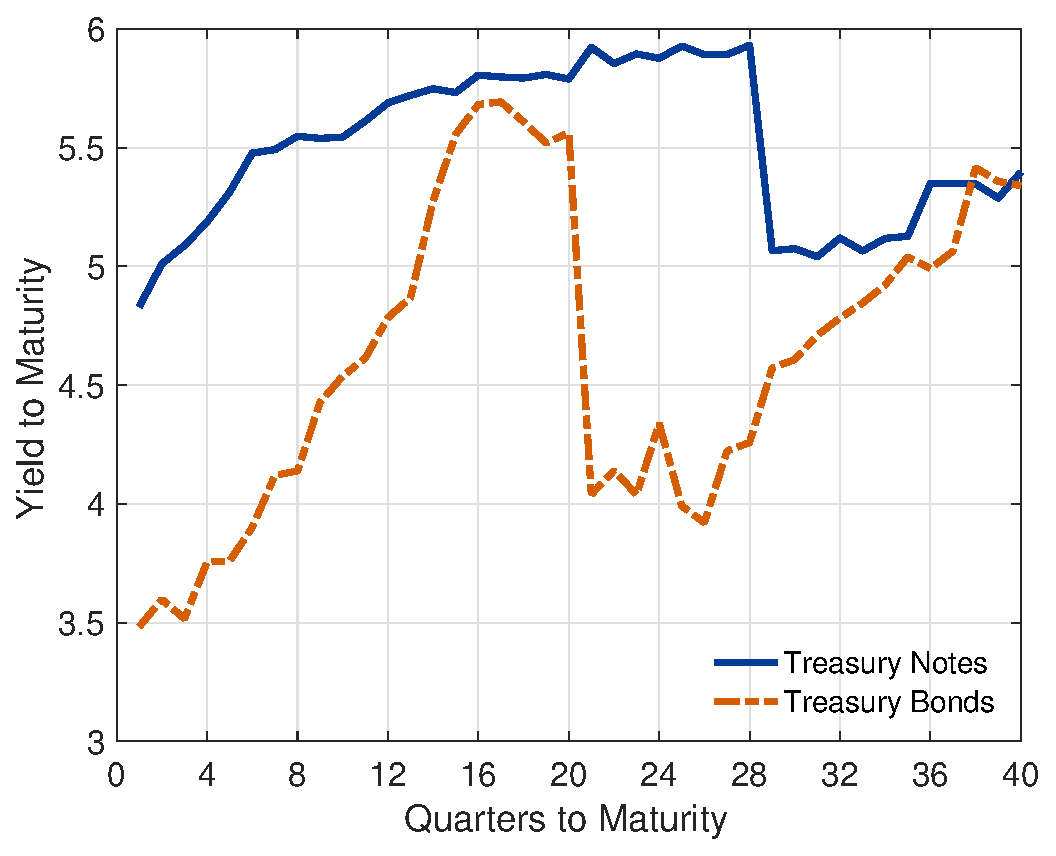
\includegraphics[width=0.7\textwidth]{../Figures/BondNote_Spread.eps}
\caption{Median Treasury Bond and Note Yields with Same Time to Maturity}{(1970-2020)}
\label{fig:YTM_Spread}
\end{figure}
%: Median YTM Time Series
% \begin{figure}[p]
% \centering
% 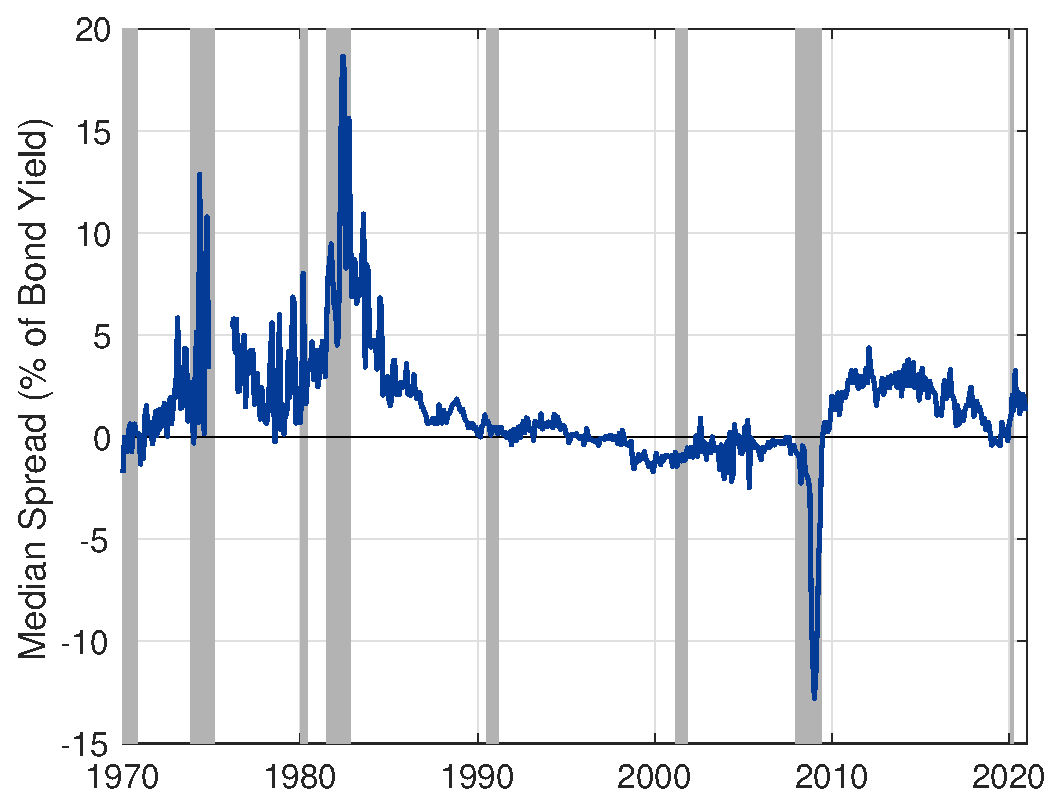
\includegraphics[width=0.7\textwidth]{../Figures/BondNote_TimeSeries.eps}
% \caption{Median Treasury Note--Bond Yield Spread with Same Time to Maturity}{(1970-2020)}
% \label{fig:YTM_SpreadTS}
% \end{figure}
%: Median Bid-Ask Spread over the Sample Period 
% \begin{figure}[p]
% \centering
% 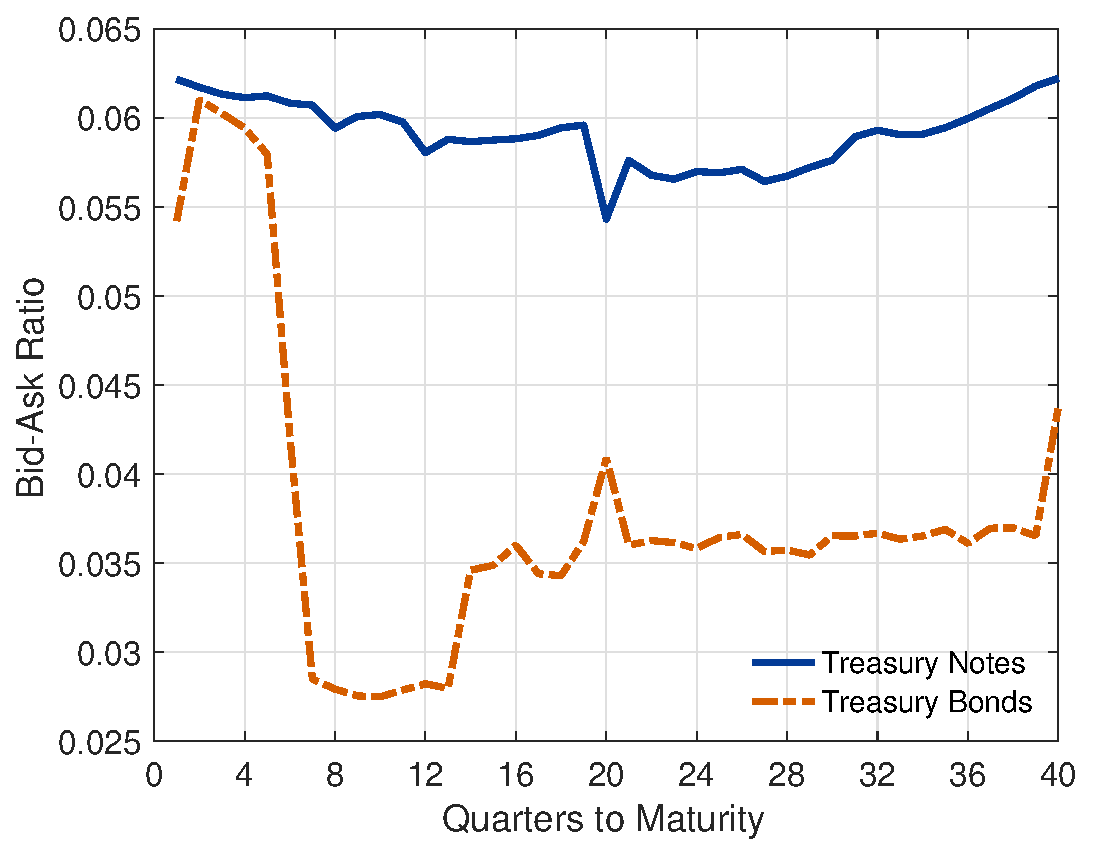
\includegraphics[width=0.7\textwidth]{../Figures/BidAsk_Ratios.eps}
% \caption{Median Treasury Bond and Note Bid-Ask Ratios with Same Time to Maturity}{(1970-2020)}
% \label{fig:BidAsk_Ratios}
% \end{figure}

\citet{Amihud-Mendelson:1991} find that the YTM spread between notes and bills is driven by relative liquidity.
Using monthly data on Treasury securities identified at the CUSIP level, I extend their work to empirically test this claim across the three common types of nominal securities.
The data are first separated by their type label: bills, notes, and bonds.
Then, for every month in the Oct 1996--Dec 2020 subsample period, each ``senior'' security (bond/note) is matched to a ``junior'' security (note/bill) that matures within one day of the respective note, allowing for exact matches.\footnote{
	The October 1996 cutoff for this analysis comes from the source data in the CRSP database. 
	Prior to October 16, 1996, CRSP data on bid and ask prices were sourced from the FRBNY; while sourced from GovPX and its aquiring institutions since then.
	According to the CRSP documentation: ``The FRBNY described its listed bid price as `...the most widely quoted price from the range of quotations received'. 
	The ask price was determined by the FRBNY based on what they expect a typical bid-ask spread to be. 
	The rule used to make this derivation was not public domain.
	GovPX described its listed bid and ask prices as the `best price'. To determine their `best price' they observe the prices from the five inter-dealer brokers and report the bid and ask prices that produce the smallest bid-ask spread.''
	Use of latter period data ensures that these irregularities in the data do not interfere with the analysis.
}
Securities without a match are removed from the analysis.
The securities' YTM spreads are then regressed against the spreads in their relative bid-ask ratios, which are calculated as 
$$ \text{relative bid-ask ratio} = \frac{\text{ask price }-\text{ bid price}}{\text{ask price }+\text{ accrued interset}}\times 100.$$
An increase in the bid--ask spread implies a relative decrease in the liquidity of the ``senior'' security.
I also control for the spread in their respective coupon rates, a general time to maturity (months/years) for any term effects, and the expected state of the economy at the time through the 10yr--2yr yield curve spread.\footnote{
	Note that the coupon rate for bills is zero.
	The 10yr--2yr spread is used because it is a spread between two notes, attempting to get at the general expectations of the future economy without crossing the asset types in the process. 
	Standard errors are heteroskedasitcally robust (HC1).
}
Table \ref{tab:Relative_Liquidity} presents the results for the notes--bills, bonds--notes, and bonds--bills analyses.

Matching the findings of \citet{Amihud-Mendelson:1991}, the differences in note and bill YTM can be explained by their relative liquidities.
That is, bills benefit from a liquidity premium and cannot be considered as perfect substitutes for notes, and vice versa.

The results of the bonds--notes and bonds--bills analyses paint bonds primarily as a savings vehicle in financial markets. 
Neither the bond's coupon rate nor the expected state of the economy impact its YTM spread versus bills, suggesting that bonds are largely purchased to hold.
Additionally, a decrease in the liquidity of bonds relative to bills causes the YTM spread to decrease, opposite of the notes result. 
A plausible explanation for this is that the demand for bonds reduces the YTM relative to bills, but that these bonds are purchased for savings purposes and are more likely held to maturity, reducing the liquidity of the market overall.
The positive, yet not statistically significant bonds-notes liquidity result also suggests that bonds occupy a part of the market that is less concerned with the liquidity of the investment and more about the safety and return.

% Notes seem to fall somewhere in the middle of the bills' liquidity hedge and the bonds' savings preference.
% The combination of results suggests that notes are less sensitive to changes in expectations, suggesting that an increase in the yield curve spread pushes bill and bond rates down together, with note rates remaining relatively unchanged.

Overall, these results confirm the generally accepted theory that bills are primarily used as a liquidity hedge while bonds are primarily a savings vehicle.
Notes seem to fall somewhere in the middle, being more sensitive to market liquidity relative to bills, and more sensative to differences in return relative to bonds.
These results also confirm that, when aggregating, none of these assets should be treated as perfect substitutes for the others.

% The relative liquidities of bonds and notes, on the other hand, do not have a statistically significant impact on their YTMs.
% The reasoning behind this result becomes more intuitive when the bonds--bills analysis is included.
% Here, an increase in bond liquidity relative to bills actually causes their YTM spread to widen; opposite of the note--bill result.
% Neither the bond's coupon rate nor the expected state of the economy has a statistically significant impact, either, counter to that of the note--bill results.
% These results become more intuitive if we think of Treasury bonds as a pure savings vehicle in international financial markets.
% In this situation, the yield--liquidity causation is reversed.
% An increase in demand for an asset that will be purchased and held rather than sold would drive down the YTM while simultaneously decreasing the liquidity in the market.
% Together, these results suggest that bills are primarily as a liquidity hedge, while bonds are primarily used as a savings vehicle.
% Notes, on the other hand, are somewhere in the middle, and none of these assets should be treated as perfect substitutes for the others.



\begin{table}[h]
	\centering
	\setlength{\tabcolsep}{15pt}
    \renewcommand{\arraystretch}{1.5}
	\caption{Relative Liquidity and Yield to Maturity$^a$} \vspace{1em}
	\label{tab:Relative_Liquidity}
	\begin{threeparttable}
		\begin{tabular}{l d{2.4} d{2.4} d{2.4}} \toprule
										& \multicolumn{1}{c}{Notes--Bills$^{b}$}  	& \multicolumn{1}{c}{Bonds--Notes} 	& \multicolumn{1}{c}{Bonds--Bills$^{b}$}	\\ \midrule
			Relative Bid-Ask Spread 	& 0.4163^{**}								& 0.0981							& -0.1424^{**}		 					\\ [-0.5em]
										& (0.173)									& (0.074)							& (0.074)	 						\\
			Coupon Rate Spread 			& 0.0210^{***}								& 0.0170^{***}						& 0.0076 							\\ [-0.5em]
										& (0.001)									& (0.005)							& (0.013)	 						\\
			Months to Maturity 			& -0.0152^{***} 							& 									& -0.1028^{***}								 	\\ [-0.5em]
										& (0.002)									&									& (0.018)									\\
			Years to Maturity 			& 											& -0.0049^{***}						& 			 					\\ [-0.5em]
										& 											& (0.001)							& 		 						\\
			% Year Dummy 					& 0.0027^{***}								& -0.0079^{***}						& -0.0079 			\\ [-0.5em]
			% 							& (0.001) 									& (0.001)							& (0.001)	 		\\ 
			10y-2y Spread 				& 0.0234^{***}								& -0.0124^{***}						& -0.0484 					\\ [-0.5em]
										& (0.003) 									& (0.002)							& (0.033)	 						\\ 
			Constant					& 0.0076 									& -0.0554^{**}						& -0.3244^{**} 						\\ [-0.5em]
										& (0.010)									& (0.030) 							& (0.154)  							\\\midrule
			Observations				& \multicolumn{1}{c}{2250}					& \multicolumn{1}{c}{7430}			& \multicolumn{1}{c}{78} 			\\
			R-Squared					& 0.207										& 0.505								& 0.399			 					\\
			F-statistic 				& 99.48										& 207.2								& 20.19			 					\\ \bottomrule 
		\end{tabular}
		\begin{tablenotes}
			\item[a] \footnotesize{The dependent variable is the yield-to-maturity spread between securities matched by thier respective days to maturity. Standard errors are heteroskedasticity robust (HC1). Designations ***, **, and * represent results that are statistivally significant at the one, five, and ten percent levels, respecitivly.}
			\item[b] \footnotesize{Analyses considering Treasury bills are limited to those securities with six months to maturity or less. This ensures that both securities have no other payments remaining until the maturity date.}
		\end{tablenotes}
	\end{threeparttable}
\end{table}




\subsection{Finding the Proper Quantity Index}
\label{subsec:Hurdles}
Given that these Treasury securities are not perfect substitutes, the next step is selecting the best quantity index for proper aggregation.
\citet{Christensen-Jorgenson-Lau:1971} show that the homogenous tanslog function 
$$ \ln f(x_t) = \alpha_0 + \sum_{n=1}^N \alpha_n \ln x^n_t + \frac{1}{2}\sum_{j,k=1}^N \gamma_{j,k} \ln x^j_t \ln x^k_t, $$
can provide a second-order approximation to an unknown, arbitrary twice-continuously-differentiable linear homogenous aggregator.
Here, $\sum_{n=1}^{N} \alpha_n = 1$, $\gamma_{j,k} = \gamma_{k,j}$, and $\sum_{k=1}^{N} \gamma_{j,k} = 0$ for $j \in [1,N]$.
\citet{Boisvert:1982} explains that the translog function is is more flexible than the Cobb-Douglas or constant elasticity of substitution (CES) functional forms by allowing the partial elastiticies of substituion between the assets to vary.
He also goes on to explain that this functional form can be viewed as a) an exact aggregator function, b) a second-order Taylor approximation to a general, but unknown aggregator function, or c) a second-order approximation to a CES function.
These properties make the translog function the perfect starting point in deriving the best quantity index.

\citet[][Section 2]{Diewert:1976} shows that the T\"{o}rnqvist-Theil Divisia quantity index 
\begin{equation*}
	\ln{M^d_t} = \ln{M^d_{t-1}} + \sum_{n=1}^{N}\frac{1}{2}(s_{n,t}+s_{n,t-1})\left(\ln{x^n_{t}} - \ln{x^n_{t-1}}\right),
	\label{DI}
\end{equation*}
can be derived directly from a translog aggregator function.
Here, $M^d_t$ is the level of the Divisia monetary aggregate, $x^n_{t}$ is the nominal value of asset $n$, and 
\begin{equation*}
	s_{n,t}  = \frac{\eta^n_{t}x^n_{t}}{\boldsymbol \eta_t \mathbf{x'}_t}
\end{equation*}
corresponds to the weight on the marginal change in financial asset $n$.
Here, $\mathbf{x}_t$ and $\boldsymbol \eta_t$ are $N \times 1$ vectors of nominal quantities and user costs, respectively.
This type of quantity index is ubiquitous in the monetary aggregation literature.

One drawback of the T\"{o}rnqvist-Theil Divisia index is that it does not handle assets coming into and out of the market ($x^n_{t} = 0$ for some $n,t$) very well.
Given the frequent changes in Treasury policy and the potential categorizations I will use, zero values are likely to be commonplace in this analysis.
When calculating general monetary aggregates, this problem does not arise often and is managed by imputing a reservation price and switching to a Fisher ideal index 
\begin{equation}
	M^f_t = M^f_{t-1}\left[\frac{(\boldsymbol \eta_t \mathbf{x'}_t) (\boldsymbol \eta_{t-1} \mathbf{x'}_t)}{(\boldsymbol \eta_t \mathbf{x'}_{t-1}) (\boldsymbol \eta_{t-1} \mathbf{x'}_{t-1})}\right]^{\frac{1}{2}}
	\label{eq:FisherIdeal}
\end{equation}
for those time periods.
\citet{Diewert:1976} shows that this quantity index is also superlative, with \citet{Diewert:1978} and \citet{Dumagan:2002} showing that the two indexes will appriximate each other numerically and mathematically, respectively.
Additionally, \citet{Diewert:1976} shows that the ideal index is derived from a quadratic mean of order 2 quantity index, which corresponds to the assumed translog aggregator function and is even recommended as the preferred index to use \citep[][Section 5]{Diewert:1976}.
Therefore, a Fisher ideal index is used in the remaining analysis.



\section{The User Cost of Treasury Securities}
\label{sec:Theory}
As \citet{Barnett:1980} outlines, aggregation theory relies on known, exact functional forms with estimable parameters.
The functions of interest are typically utility and production functions, which are often impossible to know.
This is why I rely on statistical index numbers, whose theory only relies on the existence of maximizing behavior.
From this optimizing behavior we can derive the user costs of the underlying components and bypass the unknown parameters because the resulting index numbers are not dependent on any specialized properties of the aggregator function.
That is, while I'm not deriving the true aggregate itself, the resulting quantity index will track the true aggregate.
A complete guide to index number theory and its application to monetary aggregation can be found in \citet{Barnett-Serletis:2000}.

A proper quantity index requires a price that is derived from an optimizing agent.
Thus, motivating the measurement of marketable government debt requires a partial equilibrium model that derives both the period-by-period user cost of holding government debt as well as the budgetary constraints the fiscal authority encounters.
This model incorporates both short- and long-term debt issued by the government, as well as an alternative long-term asset that acts as a pure savings vehicle and can be used as the benchmark asset. 
In this model, I refer to the alternative asset as ``capital,'' though it could also be motivated in some other fashion. 

\subsection{Long-Term Asset Dynamics}
The long-term government bonds and capital both evolve in a similar fashion.
As described by \citet{Krause-Moyen:2016}, each period new nominal long-term government bonds $B^{L,n}_t$ are issued, which are added to the stock of outstanding long-term debt $B^L_t$.
A portion $\alpha \in (0,1)$ of the previous period's stock of long-term bonds mature, while the remaining $(1-\alpha)$ remain in the stock of outstanding long-term debt. 
The maturity of these bonds is therefore $\sfrac{1}{\alpha}$.
Together, the stock of outstanding long-term debt evolves such that 
\begin{equation}
	B^L_t = (1-\alpha)B^L_{t-1} + B^{L,n}_t.
	\label{eq:LoM_DebtLevel}
\end{equation}
The average nominal interest rate paid on the stock of outstanding long-term debt $r^L_t$ evolves such that
\begin{equation}
	r^L_t B^L_t = (1-\alpha)r^L_{t-1}B^L_{t-1} + r^{L,n}_tB^{L,n}_t,
	\label{eq:LoM_DebtReturn}
\end{equation}
where $r^{L,n}_t$ is the interest rate on newly-issued long-term bonds. 

Capital is structured in a similar fashion, with the total stock of outstanding capital evolving according to
\begin{equation}
	K_t = (1-\delta)K_{t-1} + I_t,
	\label{eq:LoM_CapLevel}
\end{equation}
where $I_t$ is new investment in capital and $\delta \in (0,1)$ designates the portion of the outstanding stock of capital that matures each period.
This implies that the maturity of capital is $\sfrac{1}{\delta}$. 
The average interest rate paid on the capital stock outstanding $R_t$ is derived by
\begin{equation}
	R_tK_t = (1-\delta)R_{t-1}K_{t-1} + R^n_tI_t,
	\label{eq:LoM_CapReturn}
\end{equation}
where $R^n_t$ is the interest rate on newly-issued capital.

\subsection{Representative Household}
The representative household in this model works $l_t$ hours each period for nominal wage $W_t$.
It also earns income through it's previous investments in capital $(\delta + R_{t-1})K_{t-1}$, short-term (one-period) bonds $(1+r_t)B_{t-1}$, long-term bonds $(\alpha + r^L_{t-1})B^L_{t-1}$, and profits from a continuum of intermediate goods-producing firms $\int^1_0 \Pi_t(s) \mathrm{d}s$.\footnote{
	The $\delta$ considered here can deviate from that in (\ref{eq:LoM_CapLevel}) if depreciation is considered.
	In this present study, however, we assume zero deprecation and treat ``capital'' as an alternative long-term security similar to the long-term government bond.
	Additionally, the inclusion/exclusion of the corporate profit term does not alter the results of this partial equilibrium setup, but would be needed in a full, general equilibrium presentation.}
This income is spread between a real consumption good $c_t$ at price $p_t$ as well as new investments in nominal short-term bonds $B_t$, long-term bonds $B^{L,n}_t$, capital $I_t$, and a nominal lump sum tax $P_t\tau_t$.
Combined, the household's period-by-period budget constraint can be expressed as
\begin{multline}
	B_t + B^{L,n}_t + p_tc_t + I_t = (\delta + R_{t-1})K_{t-1} + (1+r_{t-1})B_{t-1} + \\ (\alpha + r^L_{t-1})B^L_{t-1} + W_tl_t + \int^1_0\Pi_t(s)\text{d}s - P_t\tau_t.
	\label{eq:HH_Budget}
\end{multline}

The household objective is to maximize utility over the real consumption good, the real monetary services provided by its portfolio of government bonds, and leisure
\begin{equation}
	\max\mathbb{E}_t\! \sum^\infty_{t=0} \beta^t\left\{u(c_t) + v\left(m_t\right) + x(1-l_t)\right\},
	\label{eq:HH_Utility}
\end{equation}
where $u(\cdot)$, $v(\cdot)$, and $x(\cdot)$ are increasing, concave functions.\footnote{
	The assumption of additive separability in $c_t$ and $m_t$ is stronger than the needed weakly separable assumption for this analysis.
	This is for better tractability and does not change the result in the end.}
Real monetary services are approximated using a second-order translog function
% The monetary services provided by the portfolio are captured by a constant elasticity of substitution function 
% \begin{equation}
% 	M_t = \left[\lambda^{\frac{1}{\sigma}}B_t^{\frac{\sigma-1}{\sigma}} + (1-\lambda)^{\frac{1}{\sigma}}{B^L_t}^{\frac{\sigma-1}{\sigma}}\right]^{\frac{\sigma}{\sigma-1}},
% 	\label{eq:HH_MonServices}
% \end{equation}
% where $\lambda \in [0,1]$ dictates the weight of each government debt security and $\sigma$ dictates the elasticity of substitution between the two assets.
\begin{equation}
	\ln m_t = \theta_0 + \theta_s \ln b_t + \theta_L \ln b^L_t + \frac{1}{2}\omega_{s,s} \left(\ln b_t\right)^2 + \frac{1}{2}\omega_{L,L} \left(\ln b^L_t\right)^2 + \omega_{s,L}\ln b_t \ln b^L_t.
	\label{eq:HH_MonServices}
\end{equation}

Solving the household's problem results in the following dynamic conditions:
\begin{equation}
	1 + \frac{\gamma_{2,t}}{b_t}\left(\theta_s + \omega_{s,s}\ln b_t + \omega_{s,L}\ln b^L_t\right) = \beta \mathbb{E}_t\!\left[\frac{\mu_{1,t+1}}{\mu_{1,t}}\frac{1+r_t}{\pi_{t+1}}\right],
	\label{eq:HH_manOC_B}
\end{equation}
%
\begin{multline}
	1 + \frac{\gamma_{2,t}}{b^L_t}\left(\theta_L + \omega_{L,L}\ln b^L_t + \omega_{s,L}\ln b_t\right) + \gamma_{4,t}\left(r^L_t-r^{L,n}_t\right) \\
	= \beta \mathbb{E}_t\!\left[\frac{\mu_{1,t+1}}{\mu_{1,t}}\frac{1}{\pi_{t+1}} \left\{ 1+r^L_t + (1-\alpha)\gamma_{4,t+1} \left(r^L_t-r^{L,n}_{t+1}\right)\right\}\right],
	\label{eq:HH_manOC_BL}
\end{multline}
%
and
\begin{equation}
	1 + \gamma_{3,t}\left(R_t - R^{n}_t\right)  = \beta\mathbb{E}_t\!\left[\frac{\mu_{1,t+1}}{\mu_{1,t}}\frac{1}{\pi_{t+1}}\left\{ 1 + R_{t} + (1-\delta)\gamma_{3,{t+1}}\left(R_{t} - R^{n}_{t+1}\right)\right\}\right],
	\label{eq:HH_manOC_K}
\end{equation}
The solution technique to the household's problem can be found in Appendix \ref{app:HH_Solution}.
Here, $\mu_{1,t} = u'(c_t)$, $\gamma_{2,t} = \sfrac{v'(\cdot)}{u'(\cdot)}$, and $\gamma_{3,t}$ and $\gamma_{4,t}$ are the relative prices of the long-term assets $B^L_t$ and $K_t$, respectively.
These prices evolve according to
\begin{equation}
	\gamma_{3,t} = \beta\mathbb{E}_t\!\left[\frac{\mu_{1,t+1}}{\mu_{1,t}}\frac{1}{\pi_{t+1}} \left\{1 + (1-\delta)\gamma_{3,{t+1}}\right\}\right],
	\label{eq:HH_manOC_R}
\end{equation}
%
and
\begin{equation}
	\gamma_{4,t} = \beta\mathbb{E}_t\!\left[\frac{\mu_{1,t+1}}{\mu_{1,t}}\frac{1}{\pi_{t+1}} \left\{1 + (1-\alpha)\gamma_{4,{t+1}}\right\}\right].
	\label{eq:HH_manOC_rL}
\end{equation}

The user costs of the short- and long-term bonds are 
\begin{equation}
	\eta_t = \frac{\mathbb{E}_t \Big[ \frac{\mu_{t+1}}{\mu_{t}}\frac{1}{\pi_{t+1}} \Big\{ R^n_t - (1-\delta)\gamma_{3,t+1}\Delta R^n_{t+1} - r_t \Big\}\Big]}{\mathbb{E}_t \Big[ \frac{\mu_{t+1}}{\mu_{t}}\frac{1}{\pi_{t+1}} \Big\{ 1+ R^n_t - (1-\delta)\gamma_{3,t+1}\Delta R^n_{t+1}\Big\}\Big]},
\end{equation}
and
\begin{equation}
\eta^L_t = \frac{\mathbb{E}_t \Big[ \frac{\mu_{t+1}}{\mu_{t}}\frac{1}{\pi_{t+1}} \Big\{ R^n_t  - (1-\delta)\gamma_{3,t+1}\Delta R^n_{t+1} - r^{L,n}_t + (1-\alpha)\gamma_{4,t+1}\Delta r^{L,n}_{t+1}\Big\}\Big]}{\mathbb{E}_t \Big[ \frac{\mu_{t+1}}{\mu_{t}}\frac{1}{\pi_{t+1}} \Big\{ 1+ R^n_t - (1-\delta)\gamma_{3,t+1}\Delta R^n_{t+1}\Big\}\Big]},
\label{eq:usercost_LT}
\end{equation}
respectively.
The derivations of these user costs can be found in Appendix \ref{app:usercost_derivation}.

% \subsection{Fiscal Capacity Considerations}
% \label{subsec:Theory_Capacity}
% \citet*{Brunnermeier-Merkel-Sannikov:2022} have shown that government debt constraints need to be augmented for the service flows (transaction/monetary services) that the securities provide.
% Here I expand upon this idea with the specifics of the model above, providing a deeper look at how we can ascertain those services flows in particular.\footnote{
% 	This is identical to the exercise conducted by \citet{Brunnermeier-Merkel-Sannikov:2020}, though I abstract from the bubble term to focus solely on the monetary services component.}
% Consider the simple budget constraint of the government in this model
% \begin{equation}
% 	(1+r_{t-1})\frac{B_{t-1}}{p_t} + (\alpha + r^L_{t-1})\frac{B^L_{t-1}}{p_t} = \frac{B_t}{p_t} + \frac{B^{L,n}_t}{p_t} + s_t,
% \end{equation}
% where $s_t$ is denotes the real primary surplus. 
% Now incorporate (\ref{eq:LoM_DebtLevel}) into the above equation to get
% \begin{equation}
% 	(1+r_{t-1})\frac{B_{t-1}}{p_t} + (1 + r^L_{t-1})\frac{B^L_{t-1}}{p_t} = \frac{B_t}{p_t} + \frac{B^{L}_t}{p_t} + s_t.
% \end{equation}
% Since (\ref{eq:HH_manOC_B}) and (\ref{eq:HH_manOC_BL}) must hold,
% \begin{multline}
% 	\frac{B_{t-1} + B^L_{t-1}}{p_t}(1+r_{t-1})= s_t  - (r_{t-1}^L - r_{t-1})\frac{B^L_{t-1}}{p_t} + \beta\mathbb{E}_t\left[\frac{\mu_{1,t+1}}{\mu_{1,t}} \frac{B_{t} +B^L_{t}}{p_{t+1}}(1+r_{t})\right] \\ 
% 		- \beta\mathbb{E}_t\left[\frac{\mu_{1,t+1}}{\mu_{1,t}} \frac{B^L_{t}}{p_{t+1}}(1+r_{t})\right] + \beta\mathbb{E}_t\left[\frac{\mu_{1,t+1}}{\mu_{1,t}} \frac{B^L_{t}}{p_{t+1}}(1+r^L_{t})\right] \\
% 		+  \gamma_{2,t}\left(\frac{\lambda M_t}{B_t}\right)^\frac{1}{\sigma}\frac{B_t}{p_t} +\gamma_{2,t}\left(\frac{(1-\lambda) M_t}{B^L_t}\right)^\frac{1}{\sigma}\frac{B^L_t}{p_t} \\
% 		+\beta\mathbb{E}_t\left[\frac{\mu_{1,t+1}}{\mu_{1,t}} \frac{B^L_t}{p_{t+1}}\left\{1+  (1-\alpha)\gamma_{4,t+1}\left(r^L_t - r^{L,n}_{t+1}\right)\right\}\right] - \gamma_{4,t}\left(r^L_t - r^{L,n}_t\right)\frac{B^L_t}{p_t}
% \end{multline}
% Including (\ref{eq:HH_manOC_rL}) and some rearranging, we can simplify the above equation to
% \begin{multline}
% 	\frac{B_{t-1} + B^L_{t-1}}{p_t}(1+r_{t-1})= s_t - (r_{t-1}^L - r_{t-1})\frac{B^L_{t-1}}{p_t} + \beta\mathbb{E}_t\left[\frac{\mu_{1,t+1}}{\mu_{1,t}} \frac{B_{t} +B^L_{t}}{p_{t+1}}(1+r_{t})\right] \\ 
% 		+ \beta\mathbb{E}_t\left[\frac{\mu_{1,t+1}}{\mu_{1,t}} \frac{B^L_{t}}{p_{t+1}}(1+r^L_{t} - (1-\alpha)\gamma_{4,t+1}\Delta r^{L,n}_{t+1} - r_t)\right]  \\
% 		+  \gamma_{2,t}\left(\frac{\lambda M_t}{B_t}\right)^\frac{1}{\sigma}\frac{B_t}{p_t} +\gamma_{2,t}\left(\frac{(1-\lambda) M_t}{B^L_t}\right)^\frac{1}{\sigma}\frac{B^L_t}{p_t}.
% \end{multline}

% The last two terms are of particular importance here.
% Incorporating the definition of the monetary services aggregate reduces the above expression to 
% \begin{multline}
% 	\frac{B_{t-1} + B^L_{t-1}}{p_t}(1+r_{t-1})= s_t  - (r_{t-1}^L - r_{t-1})\frac{B^L_{t-1}}{p_t} + \beta\mathbb{E}_t\left[\frac{\mu_{1,t+1}}{\mu_{1,t}} \frac{B_{t} +B^L_{t}}{p_{t+1}}(1+r_{t})\right] \\ 
% 		+ \beta\mathbb{E}_t\left[\frac{\mu_{1,t+1}}{\mu_{1,t}} \frac{B^L_{t}}{p_{t+1}}(1+r^L_{t} - (1-\alpha)\gamma_{4,t+1}\Delta r^{L,n}_{t+1} - r_t)\right] 
% 		+  \gamma_{2,t}\frac{M_t}{p_t},
% 	\label{eq:fiscalcapacity}
% \end{multline}
% where it can be shown that
% \begin{equation}
% 	\gamma_{2,t} = \left[\lambda \eta_t^{\sigma-1} + (1-\lambda)\left(\eta^L_t\right)^{\sigma-1}\right]^\frac{1}{\sigma-1}
% 	\label{eq:price_dual}
% \end{equation}
% is the price dual for the monetary services aggregate. 

% There are a couple of items to point out with regards to the above expression.
% First, fiscal capacity intuitively diminishes as long-term rates rise relative to short-term rates.
% This term is reflecting the convenience yields that the government enjoys on its short-term debt.
% Second, the fourth term on the right side suggests long-term debt can improve fiscal capacity via its longer maturity and a higher expected one-period return over the short-term debt. 
% That is, while capacity shrinks with higher long-term interest rates, demand for the debt increases with higher expected holding-period returns. 
% Lastly, fiscal capacity increases with the value of the monetary/transaction services the debt provides.
% Thus, the monetary services provided by government debt issuances is directly captured in the government's budget constraint in a similar fashion to that shown in \citet{Brunnermeier-Merkel-Sannikov:2022}.


\section{Data and Methodology}
\label{sec:DataMethodology}
In this section, I construct the Fisher ideal quantity index described in Section \ref{sec:Theory} from data compiled by the Center for Research in Securities Prices on marketable Treasury securities.
Non-marketable debt is typically held by intergovernmental agencies, and is therefore not typically considered to be a significant burden.\footnote{
	The inclusion of only publicly-held, marketable US Treasury debt would be the optimal choice here, but data restrictions keep me from assessing this.
	For instance, the CRSP data doesn't include the amount of each T-bill issuance held publicly.
	Another option could be to exclude the issuances held by the Federal Reserve, since that is the primary non-public holder of US Treasuries, but the SOMA data only goes back to 2003.
	Future research could apply this methodology to the shortened timeframe.}
The Treasury began its ``regular and predictable'' debt issuance campaign in the 1970s and data regarding the spot and forward interest rates goes back to January 1977.
Therefore the variables constructed here will cover the February 1977 to December 2020 period.

The first issue that needs to be addressed is essentially analogous to new-product bias.
As (\ref{eq:FisherIdeal}) shows, the calculation of the growth rates requires both current and lagged quantities and user costs. 
If I were to treat each issuance as a separate $m_{i,t}$, there would be distortions at issuance and maturity months.
For example, in the issuance month of $m_{i,t}$, the preceding month's yield $r_{i,t-1}$ of that particular issuance doesn't exist, which means its user cost $\eta_{i,t-1}$ also doesn't exist.
Therefore, an assumption would need to be made regarding this lagged user cost.
\citet{Feenstra:1994} and others have outlined a theoretically justified solution to this problem in which the price is set at its reservation level, where the quantity demanded would equal zero in the preceding month.\footnote{
	The Center for Financial Stability, which publishes data on Divisia monetary aggregates, delays the inclusion of new monetary assets for a few months.
	In this situation, however, the regular issuance and maturity of short-term debt make this strategy problematic.}
It's also well documented that on-the-run bonds sell at a premium over their off-the-run counterparts, suggesting $\eta_{i,t-1} > \eta_{i,t}$, but by how much?
Estimating the reservation price of each issuance in each month over the sample period would seem to be too technically burdensome. 
With how distortionary this bias can be, some adjustments and/or assumptions are needed.

To reduce the magnitude of this issue, I cluster the assets into groups that are most likely to be perfect substitutes in any given month.
While there may be discrepancies in on-the-run/off-the-run securities, they should average out within the clusters. 
Based on the work of \citet{Amihud-Mendelson:1991} as well as the results in Table \ref{tab:Relative_Liquidity}, the securities need to be separated across their designation of {\em bills}, {\em notes}, and {\em bonds}.
Since 1997, the Treasury has issued Treasury Inflation-Protected Securities (TIPS), which yield a real rate of interest instead of the traditional nominal yield.
These have been shown to be less liquid than their nominal counterparts, so I create two additional categories of {\em TIPS notes} and {\em TIPS bonds}. 
Lastly, as these securities mature, their yields tend to fall with the trend of the constant maturity yield curve, reflecting the changing monetary services they provide.
Therefore, each of these five categories needs to be further segmented by their time to maturity.
Since bonds and longer notes are issued on a quarterly basis, it's common to have individual months where there are no securities of a certain type.\footnote{
	These notes and bonds are typically subject to reopenings in the months following the initial issuance, but the maturity dates are unchanged.
	For example, if a 30-year bond is issued in February, a reopening of that issuance may be offered in March, but the time-to-maturity on that reopening is 29 years, 11 months.}
A fine-grained segmentation such as this would again be subject to a large amount of new-product bias, so I define each sub-category as the quarters-to-maturity.
That is, for securities that will mature over the next one-to-three months, they are categorized has maturing within one quarter. 
A thirty-year threshold on bonds suggests 120 quarters-worth of categories, but there were a series of longer-term bonds that were issued between 1953 and 1965, which could impact the first years of the analysis.
Therefore, the number of quarters-to-maturity categories is set at 160, or forty years. 
Overall, when accounting for both the types of securities and the quarters to maturity, there are 800 categories.\footnote{
	Note that, based on (\ref{eq:FisherIdeal}), baskets that are consistently empty do not impact the measurement, allowing me to keep it consistent across the types of securities.
	So while there are 800 total baskets, a large number of them will not contribute to the measurement, but it does provide the flexibility needed for the aggregate over the almost fifty-year analysis.}
	
The next step in this process is to identify the proper interest rates from the theory above.
Since the user costs represent the holding period return and incorporate the interest rates paid on newly-issued securities ($r_t$ and $r^{L,n}_t$) and not on the average interest rate paid out on outstanding debt ($r^L_t$), the most accurate interest rates to consider are the coupon rates.
Additionally, the term $(1-\alpha)\gamma_{4,t+1}\Delta r^{L,n}_{t+1}$ represents the expected capital gains of the long-term bond. 
To account for these expectations, I use the current price of the bonds adjusted for its maturity, multiplied by the difference between the one-month-ahead forward rate and spot rate for each bond's particular month and maturity.
For TIPS, I consider the real spot and forward yield curves in the calculation of expected capital gains. 
While forward rates incorporate more than just future expectations of current spot rates, the impact of any term premium looking only one month ahead should be negligible.

The rate considered for each basket of securities is the quantity-weighted average over the issuances therein, though a further assumption is needed to address missing values/new-product bias.
As discussed above, even the broader categories used here do not ensure that there are no issues with new-product bias.
Since most of the empty categories in this situation are simply a cluster of maturing debt through time, and not new issuances of debt, I use the linear interpolation of the rates across the maturities instead of calculating a reservation rate.
This ensures that I'm capturing the true shape of the yield curves used. 

The benchmark rate used here is the maximum holding-period return of the baskets of securities considered each month, plus twenty-five basis points.\footnote{
	Previous iterations of this measurement attempted to use the Baa Corporate Bond yield, which would have accounted for both the liquidity and safety attributes of Treasury securities.
	However, even the addition of 200 basis points did not ensure that all user costs were positive across the sample period, especially in the volatile years of 1979--1981 and long periods of time between 2014 and 2016.
	Adjustments to create that kind of spread for the early years also had the drawback of washing out the differences in user costs in the later parts of the sample period.}
This is similar to the strategy used by the Federal Reserve in their calculation of Divisia monetary aggregates and is common in other derivations of user costs. 

\section{Results}
\label{sec:Results}

\subsection{The Measure}
\label{subsec:Results_Measure}

The Fisher ideal quantity index of US fiscal debt---and its corresponding simple-sum aggregate---is presented in Figure \ref{fig:MS_Index}.
This value is constructed from the month-over-month growth rates calculated via the logarithm of (\ref{eq:FisherIdeal}).\footnote{
	This indirect approach to the aggregates' levels is necessary as there is no initial value from which to begin the calculation of (\ref{eq:FisherIdeal}).
	These month-over-month growth rates can be found in Appendix \ref{app:Additional_Results}.
}
Multiple theories have claimed that Treasury securities provide services above and beyond their principal value, but this is the first attempt to measure such services. 
The base month considered here is August 1989 due to the relative flatness of the yield curve at that time.
When the yield curve is flat, the differences in the user costs are minimal, suggesting that the underlying assets are perceived as near-perfect substitutes and collapsing the Fisher ideal index into a simple sum aggregate. 
%: Simple sum versus Fisher index
\begin{figure}[h]
	\centering
	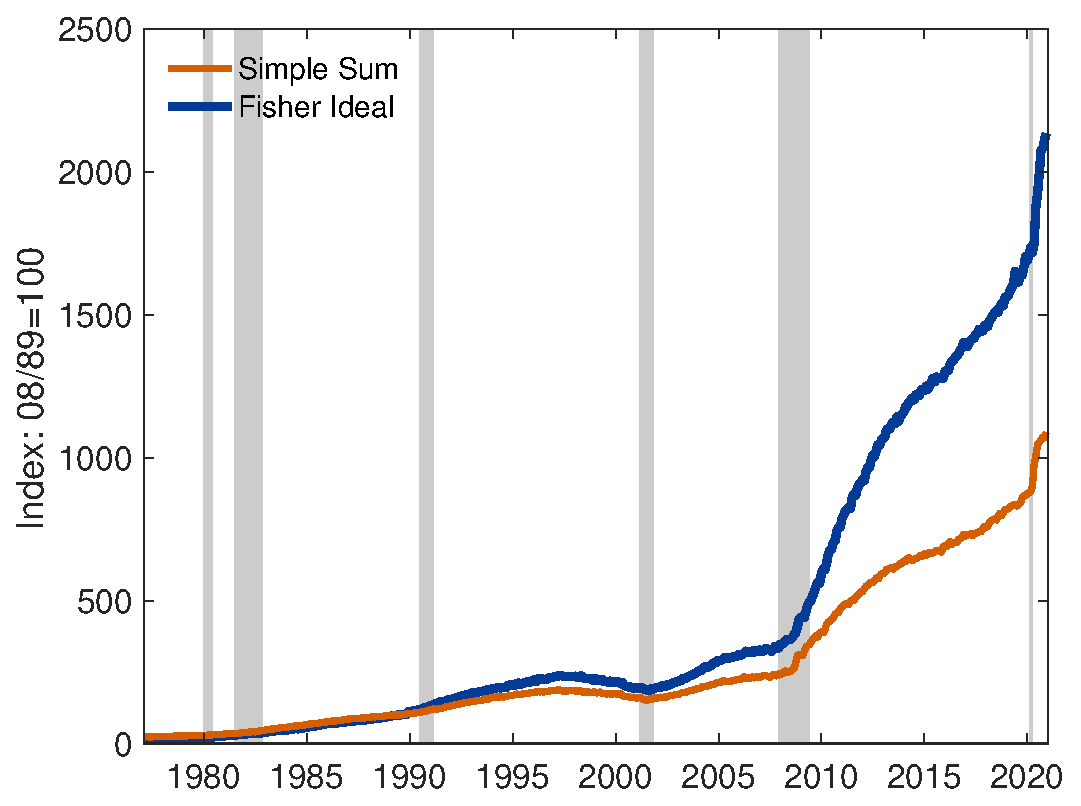
\includegraphics[width=0.85\textwidth]{../Figures/FisherIndex_v2.eps}
	\caption{Monetary Services Level}
	\label{fig:MS_Index}
\end{figure}
%: Differences in the Aggregates' Growth Rates
% \begin{figure}[h]
% 	\centering
% 	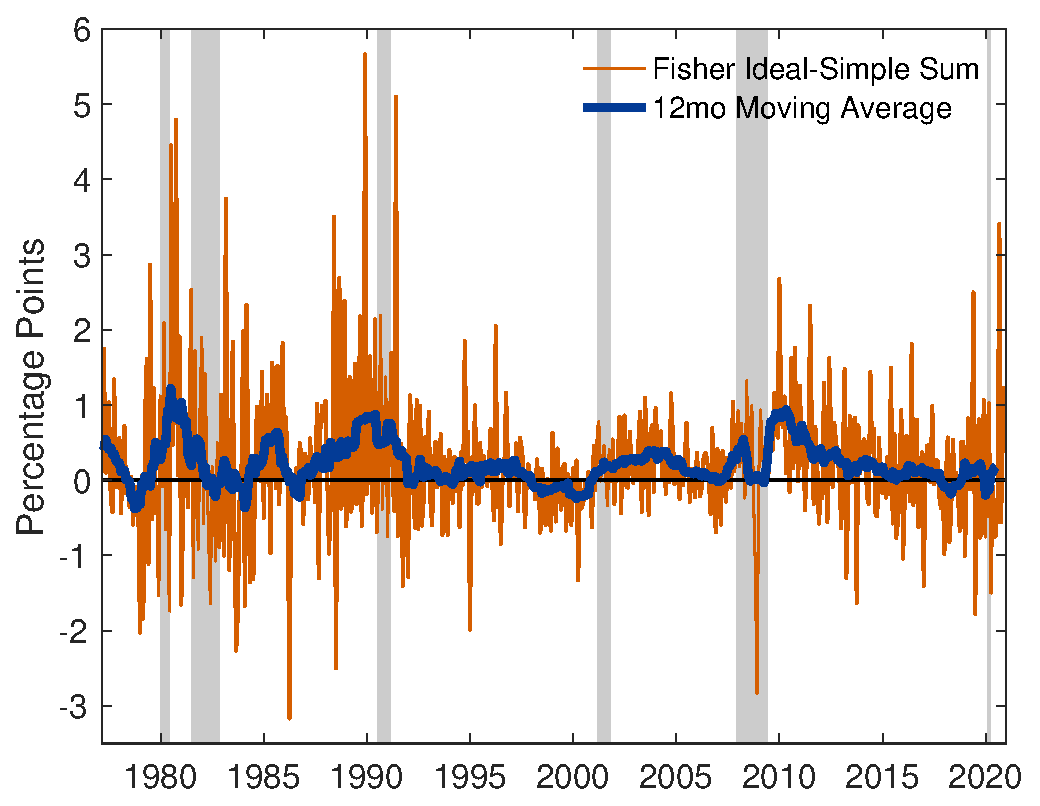
\includegraphics[width=0.85\textwidth]{../Figures/GrowthDiff_v2.eps}
% 	\caption{Month-over-month Growth Rate Spread}
% 	\label{fig:Growth_Spread}
% \end{figure}
Using the respective growth rates of both measures, I estimate the growth rate of the fiscally-supplied monetary services.
Since the true aggregate incorporates both the quantities of the underlying assets and the monetary services they provide, the difference in their growth rates reveals the growth of the monetary services alone.
That is, I am essentially factoring-out the growth that comes purely from the issued principal values.
This series is then used to constuct a quantity index for the monetary services (Figure \ref{fig:MS_Index}), separated from the quantity of the underlying principal value.
%: Index Values of the Monetary Services
\begin{figure}[p!]
	\centering
	\includegraphics[width=0.85\textwidth]{../Figures/MonetaryServices_Index.eps}
	\caption{Derived Monetary Services Quantity Index}
	\label{fig:MS_Index}
\end{figure}
As can be seen, these monetary services have generally grown as principal levels have risen, though it is not uncommon for the monetary services of fiscal debt to decrease even in the face of deficit spending.
The year-over-year growth rate of these monetary services is easier to analyze and shown in Figure \ref{fig:YoY_Growth}.
\begin{figure}[p!]
	\centering
	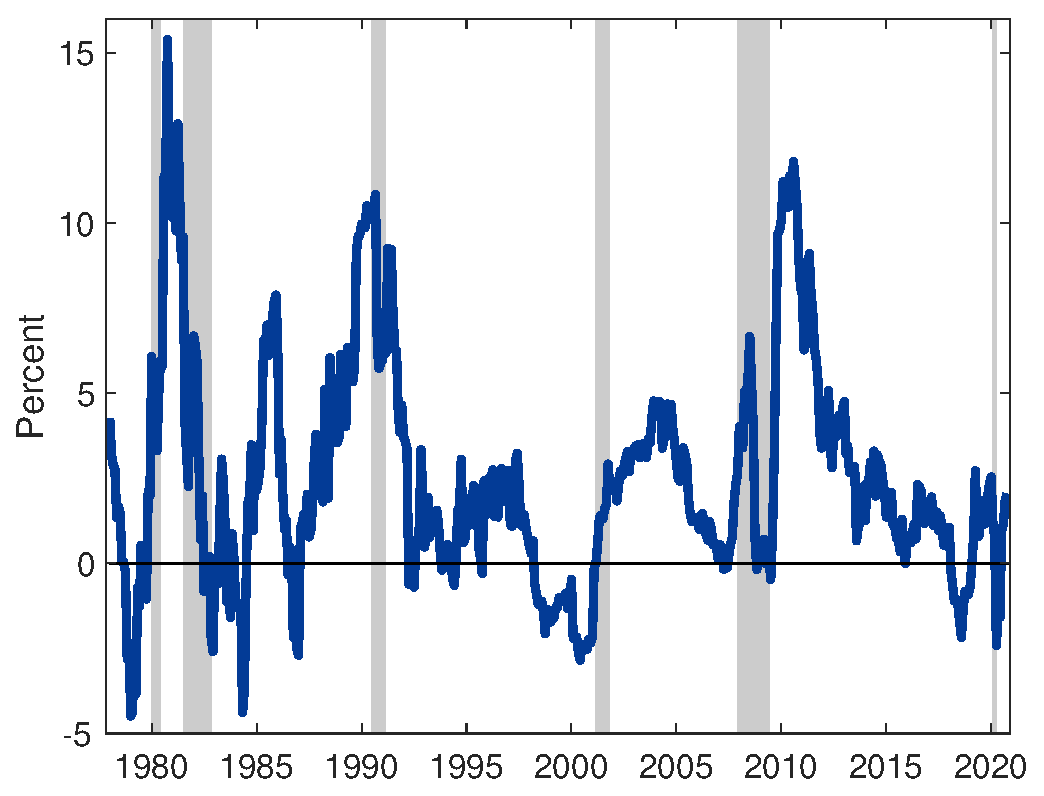
\includegraphics[width=0.85\textwidth]{../Figures/YoYGrowth_MonServices.eps}
	\caption{Year-over-year Growth of Fiscally-Supplied Monetary Services}
	\label{fig:YoY_Growth}
\end{figure}


% The spread in Figure \ref{fig:Growth_Spread}, therefore, represents the growth of fiscally-provided monetary services.
% This figure shows us that the Treasury generally adds to the stock of monetary services over time, with notable exceptions in the late-1990s when the government was running a fiscal surplus.
% In that instance, the growth rates suggest that the monetary services provided were shrinking along with the principal values. 



% Using these growth rate spreads, I derive an index that tracks the stock of monetary services, shown in Figure \ref{fig:MS_Index}.


\section{Fiscal Capacity: Accounting vs.\ Economic Value}
Discussions of fiscal debt often turn into discussions of fiscal capacity.
Focusing on the simple-sum value of the underlying principal, however, considers only the purely accounting aspects of fiscal capacity.
In this section I consider the differences between the accounting (simple-sum) approach and an approach that considers the economic value of the debt (index-number).

\subsection{Fiscal Capacity Considerations}
\label{subsec:Theory_Capacity}
\citet*{Brunnermeier-Merkel-Sannikov:2022} have shown that government debt constraints need to be augmented for the service flows (transaction/monetary services) that the securities provide.
Here I expand upon this idea with the specifics of the model above, providing a deeper look at how we can ascertain those services flows in particular.\footnote{
	This is identical to the exercise conducted by \citet{Brunnermeier-Merkel-Sannikov:2020}, though I abstract from the bubble term to focus solely on the monetary services component.}

	Consider the simple budget constraint of a government that corresponds to the household side of the model above
\begin{equation*}
	(1+r_{t-1})\frac{B_{t-1}}{p_t} + (\alpha + r^L_{t-1})\frac{B^L_{t-1}}{p_t} = \frac{B_t}{p_t} + \frac{B^{L,n}_t}{p_t} + s_t,
\end{equation*}
where $s_t$ is denotes the real primary surplus. 
Now incorporate (\ref{eq:LoM_DebtLevel}) into the above equation to get
\begin{equation}
	(1+r_{t-1})\frac{B_{t-1}}{p_t} + (1 + r^L_{t-1})\frac{B^L_{t-1}}{p_t} = \frac{B_t}{p_t} + \frac{B^{L}_t}{p_t} + s_t.
	\label{eq:Gov_PeriodBudget}
\end{equation}

For simplicity and without loss of generality, I assume that the true monetary services aggregate is a constant elastisticy of subsitution function
\begin{equation}
	M_t = \left[\lambda^{\frac{1}{\sigma}}B_t^{\frac{\sigma-1}{\sigma}} + (1-\lambda)^{\frac{1}{\sigma}}{B^L_t}^{\frac{\sigma-1}{\sigma}}\right]^{\frac{\sigma}{\sigma-1}},
	\label{eq:MS_CES}
\end{equation}
where $\lambda \in [0,1]$ dictates the weight of each government debt security and $\sigma$ dictates the elasticity of substitution between the two assets.


The equilibrium conditions analogous to (\ref{eq:HH_manOC_B}) and (\ref{eq:HH_manOC_BL})
\begin{equation*}
	1 - \gamma_{2,t}\left(\frac{\lambda M_t}{B_t}\right)^\frac{1}{\sigma} = \beta \mathbb{E}_t\!\left[\frac{\mu_{1,t+1}}{\mu_{1,t}}\frac{1+r_t}{\pi_{t+1}}\right],
	\label{eq:HH_manOC_B_Alt}
\end{equation*}
and 
\begin{multline*}
	1 - \gamma_{2,t}\left(\frac{(1-\lambda)M_t}{B^L_t}\right)^\frac{1}{\sigma} + \gamma_{4,t}\left(r^L_t-r^{L,n}_t\right) \\
	= \beta \mathbb{E}_t\!\left[\frac{\mu_{1,t+1}}{\mu_{1,t}}\frac{1}{\pi_{t+1}} \left\{ 1+r^L_t + (1-\alpha)\gamma_{4,t+1} \left(r^L_t-r^{L,n}_{t+1}\right)\right\}\right],
	\label{eq:HH_manOC_BL_Alt}
\end{multline*}
must therefore hold.
Incorporating these into (\ref{eq:Gov_PeriodBudget}) yields
\begin{multline}
	\frac{B_{t-1} + B^L_{t-1}}{p_t}(1+r_{t-1})= s_t  - (r_{t-1}^L - r_{t-1})\frac{B^L_{t-1}}{p_t} + \beta\mathbb{E}_t\left[\frac{\mu_{1,t+1}}{\mu_{1,t}} \frac{B_{t} +B^L_{t}}{p_{t+1}}(1+r_{t})\right] \\ 
		- \beta\mathbb{E}_t\left[\frac{\mu_{1,t+1}}{\mu_{1,t}} \frac{B^L_{t}}{p_{t+1}}(1+r_{t})\right] + \beta\mathbb{E}_t\left[\frac{\mu_{1,t+1}}{\mu_{1,t}} \frac{B^L_{t}}{p_{t+1}}(1+r^L_{t})\right] \\
		+  \gamma_{2,t}\left(\frac{\lambda M_t}{B_t}\right)^\frac{1}{\sigma}\frac{B_t}{p_t} +\gamma_{2,t}\left(\frac{(1-\lambda) M_t}{B^L_t}\right)^\frac{1}{\sigma}\frac{B^L_t}{p_t} \\
		+\beta\mathbb{E}_t\left[\frac{\mu_{1,t+1}}{\mu_{1,t}} \frac{B^L_t}{p_{t+1}}\left\{1+  (1-\alpha)\gamma_{4,t+1}\left(r^L_t - r^{L,n}_{t+1}\right)\right\}\right] - \gamma_{4,t}\left(r^L_t - r^{L,n}_t\right)\frac{B^L_t}{p_t}
\end{multline}
Subsituting (\ref{eq:HH_manOC_rL}) into this---and some rearranging---we can simplify the above equation to
\begin{multline}
	\frac{B_{t-1} + B^L_{t-1}}{p_t}(1+r_{t-1})= s_t - (r_{t-1}^L - r_{t-1})\frac{B^L_{t-1}}{p_t} + \beta\mathbb{E}_t\left[\frac{\mu_{1,t+1}}{\mu_{1,t}} \frac{B_{t} +B^L_{t}}{p_{t+1}}(1+r_{t})\right] \\ 
		+ \beta\mathbb{E}_t\left[\frac{\mu_{1,t+1}}{\mu_{1,t}} \frac{B^L_{t}}{p_{t+1}}(1+r^L_{t} - (1-\alpha)\gamma_{4,t+1}\Delta r^{L,n}_{t+1} - r_t)\right]  \\
		+  \gamma_{2,t}\left(\frac{\lambda M_t}{B_t}\right)^\frac{1}{\sigma}\frac{B_t}{p_t} +\gamma_{2,t}\left(\frac{(1-\lambda) M_t}{B^L_t}\right)^\frac{1}{\sigma}\frac{B^L_t}{p_t}.
\end{multline}

The last two terms are of particular importance here.
The assumed-true monetary services aggregate (\ref{eq:MS_CES}) reduces the above expression to 
\begin{multline}
	\frac{B_{t-1} + B^L_{t-1}}{p_t}(1+r_{t-1})= s_t  - (r_{t-1}^L - r_{t-1})\frac{B^L_{t-1}}{p_t} + \beta\mathbb{E}_t\left[\frac{\mu_{1,t+1}}{\mu_{1,t}} \frac{B_{t} +B^L_{t}}{p_{t+1}}(1+r_{t})\right] \\ 
		+ \beta\mathbb{E}_t\left[\frac{\mu_{1,t+1}}{\mu_{1,t}} \frac{B^L_{t}}{p_{t+1}}(1+r^L_{t} - (1-\alpha)\gamma_{4,t+1}\Delta r^{L,n}_{t+1} - r_t)\right] 
		+  \gamma_{2,t}\frac{M_t}{p_t},
	\label{eq:fiscalcapacity}
\end{multline}
where it can be shown that
\begin{equation}
	\gamma_{2,t} = \left[\lambda \eta_t^{\sigma-1} + (1-\lambda)\left(\eta^L_t\right)^{\sigma-1}\right]^\frac{1}{\sigma-1}
	\label{eq:price_dual}
\end{equation}
is the price dual for the monetary services aggregate. 

There are a couple of items to point out with regards to the above expression.
First, fiscal capacity intuitively diminishes as long-term rates rise relative to short-term rates.
This term is reflecting the convenience yields that the government enjoys on its short-term debt.
Second, the fourth term on the right side suggests long-term debt can improve fiscal capacity via its longer maturity and a higher expected one-period return over the short-term debt. 
That is, while capacity shrinks with higher long-term interest rates, demand for the debt increases with higher expected holding-period returns. 
Lastly, fiscal capacity increases with the value of the monetary/transaction services the debt provides.
Thus, the monetary services provided by government debt issuances is directly captured in the government's budget constraint in a similar fashion to that shown in \citet{Brunnermeier-Merkel-Sannikov:2022}.
Fiscal capacity analysis that focuses only on the accounting view of fiscal debt and omits the economic value of the underlying securities will inevitably lead to a biased view of the fiscal situation.

Fisher's factor reversal can be used to calculate the non-parametric version of the price dual (\ref{eq:price_dual}) and is shown in Figure \ref{fig:FiscalServices_Value}.
The data does not go back far enough to know whether the higher values in the late 1970s are a one-off spike or a sustained trend. 
The sudden decrease in this index in the 1989--1990 period comes from a sudden decrease in the price of obtaining these monetary services.
While the reasoning for this dramatic shift is beyond the scope of this paper, this does generally align with some later estimates of the Great Moderation as well as the surge in the information technology realm.\footnote{
	While most of the work on the Great Moderation centers around 1984:Q4 as the break point, \citet{Stock-Watson:2002} find a relatively wide 95\% confidence interval that expands all the way to 1989:Q4.
	The first web browser was also introduced in 1990, providing information in an easy-to-use format to the masses.}
One could imagine that the decrease in general market volatility, coupled with an increase in the available information about other financial assets, decimated the Treasury's comparative advantage in safety in the financial world.
\begin{figure}[h!]
\centering
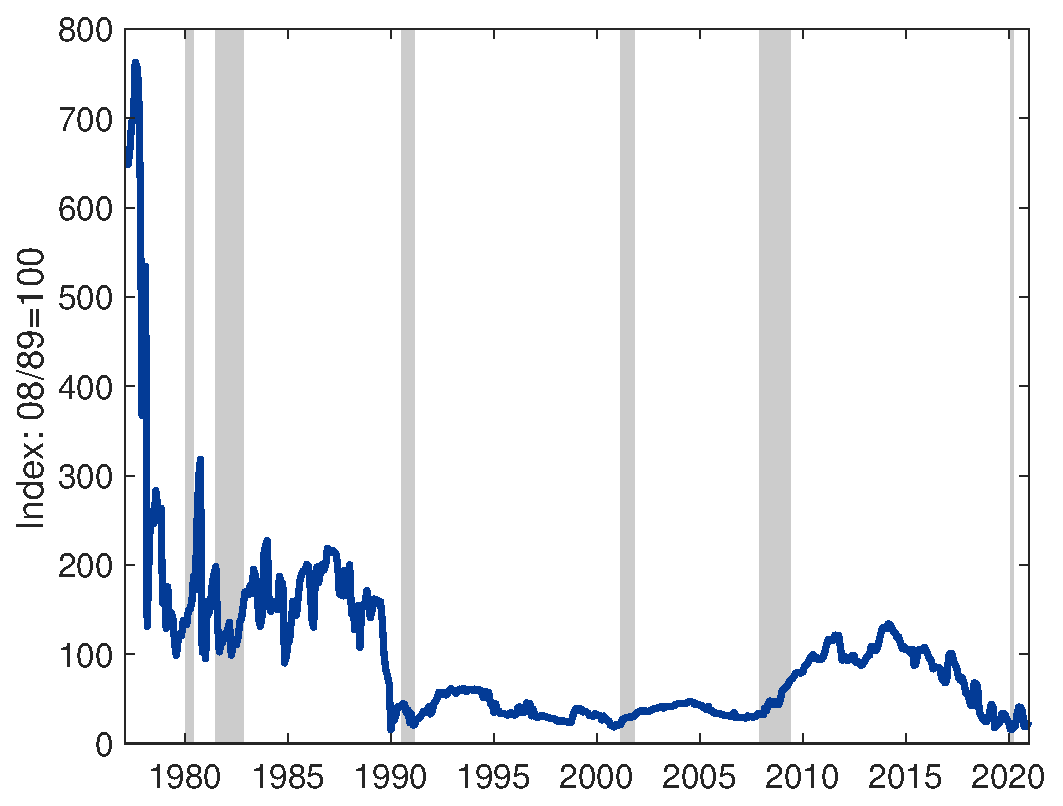
\includegraphics[width=0.85\textwidth]{../Figures/FiscalCapacity_Index.eps}
\caption{Value of Fiscal Monetary Services}
\label{fig:FiscalServices_Value}
\end{figure}

The value of the monetary services aggregate was relatively stable until the financial crisis of 2007-2009, when that value increased approximately 378 percent from January 2007 to January 2014. 
This increase in the fiscal capacity would help explain the lack of inflationary pressure during that period of expansion despite increases in federal spending and monetary stimulus over that time.
The stimulus passed during the 2020 pandemic, however, did not provide the same increase in total value, as the private sector moved towards pure liquidity (``dash for cash'') in the face of lockdowns.
In that type of environment, even Treasury securities do not provided the needed liquidity and safety features.

\section{Concluding Remarks}
The three primary contributions of this paper center around how we view fiscal debt.
First, I show empirically and theoretically that these securities should not be treated as perfect substitutes and therefore cannot be aggregated in a simple-sum manner. 
Next, I motivate the use of index number theory to account for this imperfect subsitutability; deriving the user cost for fiscal debt securities and creating a Fisher ideal quantity index.
Lastly, I reveal that a failure to account for the monetary services provided by fiscal debt ultimately leads to a misunderstanding of a nation's fiscal capacity. 

There are a multitude of extentions to this, including the calculation of indices for countries outside the United States.
Of particular interest, if the data exist, would be countries that have undergone sovereign debt crises in the recent past.
This would include countries such as Mexico, Argentina, and others, where an index like this may capture the erosion of the fiscal space better than the standard metrics.
Additionally, one simplifying assumption taken here is that of risk neutrality or perfect certainty.
While Treasury securities are considered to be the safest assets on the market, the inclusion of capital gains in the user costs means that there will always be some risk involved.
An extension of this work, therfore, would be to derive the user costs under risk as \citet{Barnett-Liu-Jensen:1997} do for monetary aggregates.

In an economic and political environment in which fiscal debt is growing more and more salient, understanding how to properly track the metrics of choice and how they fit within the bigger picture becomes even more important.
This paper shows how to view fiscal debt beyond simple accounting and why considering the true economic value of fiscal debt is important for future policy decisions. 
\newpage

\bibliographystyle{apecon}
\bibliography{MonetaryServices_Debt}

\newpage
\appendix
\numberwithin{equation}{section}
\section{Representative Household Solution}
\label{app:HH_Solution}

Combining (\ref{eq:LoM_DebtLevel}) and (\ref{eq:LoM_DebtReturn})
\begin{equation}
	\left(r^L_t-r^{L,n}_t\right)B^L_t = (1-\alpha)\left(r^L_{t-1}-r^{L,n}_t\right)B^L_{t-1},
	\label{eq:CombEq_1}
\end{equation}
(\ref{eq:LoM_CapLevel}) and (\ref{eq:LoM_CapReturn})
\begin{equation}
	\left(R_t-R^{n}_t\right)K_t = (1-\delta)\left(R_{t-1}-R^{n}_t\right)K_{t-1},
	\label{eq:CombEq_2}
\end{equation}
and (\ref{eq:HH_Budget}), (\ref{eq:LoM_DebtLevel}), and (\ref{eq:LoM_CapLevel})
\begin{multline}
	B_t + B^{L}_t - (1-\alpha)B^L_{t-1} + p_tc_t + K_t - (1-\delta)K_{t-1} = (\delta + R_{t-1})K_{t-1} \\+ (1+r_{t-1})B_{t-1} + (\alpha + r^L_{t-1})B^L_{t-1} + W_tl_t + \int^1_0\Pi_t(s)\text{d}s - P_t\tau_t.
	\label{eq:CombEq_3}
\end{multline}

\subsection{Household's Problem}
(\ref{eq:HH_Utility}) subject to (\ref{eq:HH_MonServices}), (\ref{eq:CombEq_1}), (\ref{eq:CombEq_2}), and (\ref{eq:CombEq_3}). Choosing 
$\left\{B_t, B^L_t, c_t, K_t, R_t, r^L_t, l_t, M_t\right\}$

\subsection{Bellman Equation}

\begin{multline}
	\mathbb{V}\!\left(B_{t-1}, B^L_{t-1}, K_{t-1}, R_{t-1}, r^L_{t-1}\right) \\= \max \Bigg\{u(c_t) + v\left(\frac{M_t}{P_t}\right) + x(l_t)  + \beta\mathbb{E}_t\!\left[\mathbb{V}\!\left(B_{t}, B^L_{t}, K_{t}, R_{t}, r^L_{t}\right)\right] \\
	+ \frac{\mu_{1,t}}{p_t} \Big[(\delta + R_{t-1})K_{t-1} + (1+r_{t-1})B_{t-1} + (\alpha + r^L_{t-1})B^L_{t-1} + W_tl_t \\+ \int^1_0\Pi_t(s)\text{d}s -P_t\tau_t -B_t - B^{L}_t + (1-\alpha)B^L_{t-1} - p_tc_t - K_t + (1-\delta)K_{t-1}\Big] \\
	+ \frac{\mu_{2,t}}{p_t}\Bigg[\theta_0 + \theta_s \ln b_t + \theta_L \ln b^L_t + \frac{1}{2}\omega_{s,s} \left(\ln b_t\right)^2 + \frac{1}{2}\omega_{L,L} \left(\ln b^L_t\right)^2 + \omega_{s,L}\ln b_t \ln b^L_t-\ln m_t\Bigg] \\
	+ \frac{\mu_{3,t}}{p_t}\Big[(1-\delta)\left(R_{t-1}-R^{n}_t\right)K_{t-1} - \left(R_t-R^{n}_t\right)K_t \Big] \\
	+ \frac{\mu_{4,t}}{p_t} \Big[(1-\alpha)\left(r^L_{t-1}-r^{L,n}_t\right)B^L_{t-1} - \left(r^L_t-r^{L,n}_t\right)B^L_t\Big]\Bigg\}
	\label{eq:Bellman}
\end{multline}

\subsection{First Order Conditions}

\begin{equation}
	u'(c_t) = \mu_{1,t}
	\label{eq:HH_FOC_c}
\end{equation}
%
\begin{equation}
	v'\left(m_t\right) = \mu_{2,t}
	\label{eq:HH_FOC_M}
\end{equation}
%
\begin{equation}
	x'(1-l_t) = -\mu_{1,t}w_t
	\label{eq:HH_FOC_l}
\end{equation}
%
\begin{equation}
	\beta\mathbb{E}_t\!\left[\mathbb{V}\!_1\left(B_{t}, B^L_{t}, K_{t}, R_{t}, r^L_{t}\right)\right] = \frac{\mu_{1,t}}{p_t} + \mu_{2,t}\left[\theta_s\frac{1}{B_t} + \omega_{s,s}\ln b_t \frac{1}{B_t} + \omega_{s,L}\ln b^L_t \frac{1}{B_t}\right]
	\label{eq:HH_FOC_B}
\end{equation}
%
\begin{equation}
	\beta\mathbb{E}_t\!\left[\mathbb{V}\!_2\left(B_{t}, B^L_{t}, K_{t}, R_{t}, r^L_{t}\right)\right] = \frac{\mu_{1,t}}{p_t} + \mu_{2,t}\left[\theta_L\frac{1}{B^L_t} + \omega_{L,L}\ln b^L_t \frac{1}{B^L_t} + \omega_{s,L}\ln b_t \frac{1}{B^L_t}\right]
	\label{eq:HH_FOC_BL}
\end{equation}
%
\begin{equation}
	\beta\mathbb{E}_t\!\left[\mathbb{V}\!_3\left(B_{t}, B^L_{t}, K_{t}, R_{t}, r^L_{t}\right)\right] = \frac{\mu_{1,t}}{p_t} + \frac{\mu_{3,t}}{p_t}\left(R_t - R^{n}_t\right)
	\label{eq:HH_FOC_K}
\end{equation}
%
\begin{equation}
	\beta\mathbb{E}_t\!\left[\mathbb{V}\!_4\left(B_{t}, B^L_{t}, K_{t}, R_{t}, r^L_{t}\right)\right] = \frac{\mu_{3,t}}{p_t}K_t
	\label{eq:HH_FOC_R}
\end{equation}
%
\begin{equation}
	\beta\mathbb{E}_t\!\left[\mathbb{V}\!_5\left(B_{t}, B^L_{t}, K_{t}, R_{t}, r^L_{t}\right)\right] = \frac{\mu_{4,t}}{p_t}B^L_t
	\label{eq:HH_FOC_rL}
\end{equation}

\subsection{Bienveniste-Scheinkman Conditions}

\begin{equation}
	\mathbb{V}\!_1\left(B_{t-1}, B^L_{t-1}, K_{t-1}, R_{t-1}, r^L_{t-1}\right) = \frac{\mu_{1,t}}{p_t}(1+r_{t-1})
	\label{eq:HH_BS_B}
\end{equation}
%
\begin{equation}
	\mathbb{V}\!_2\left(B_{t-1}, B^L_{t-1}, K_{t-1}, R_{t-1}, r^L_{t-1}\right) = \frac{\mu_{1,t}}{p_t}(1+r^L_{t-1}) + \frac{\mu_{4,t}}{p_t}(1-\alpha)\left(r^L_{t-1} - r^{L,n}_t\right)
	\label{eq:HH_BS_BL}
\end{equation}
%
\begin{equation}
	\mathbb{V}\!_3\left(B_{t-1}, B^L_{t-1}, K_{t-1}, R_{t-1}, r^L_{t-1}\right) = \frac{\mu_{1,t}}{p_t}(1 + R_{t-1}) + \frac{\mu_{3,t}}{p_t}(1-\delta)\left(R_{t-1} - R^{n}_t\right)
	\label{eq:HH_BS_K}
\end{equation}
%
\begin{equation}
	\mathbb{V}\!_4\left(B_{t-1}, B^L_{t-1}, K_{t-1}, R_{t-1}, r^L_{t-1}\right) = \left(\frac{\mu_{1,t}}{p_t} + (1-\delta)\frac{\mu_{3,t}}{p_t}\right)K_{t-1}
	\label{eq:HH_BS_R}
\end{equation}
%
\begin{equation}
	\mathbb{V}\!_5\left(B_{t-1}, B^L_{t-1}, K_{t-1}, R_{t-1}, r^L_{t-1}\right) = \left(\frac{\mu_{1,t}}{p_t} + (1-\alpha)\frac{\mu_{4,t}}{p_t}\right)B^L_{t-1}
	\label{eq:HH_BS_rL}
\end{equation}

\subsection{Optimality Conditions}

\begin{equation}
	u'(c_t) = \mu_{1,t}
	\label{eq:HH_OC_c}
\end{equation}
%
\begin{equation}
	v'\left(\frac{M_t}{p_t}\right) = \mu_{2,t}
	\label{eq:HH_OC_M}
\end{equation}
%
\begin{equation}
	x'(1-l_t) = -\mu_{1,t}w_t
	\label{eq:HH_OC_l}
\end{equation}
%
\begin{equation}
	1 + \frac{\gamma_{2,t}}{b_t}\left(\theta_s + \omega_{s,s}\ln b_t + \omega_{s,L}\ln b^L_t\right) = \beta \mathbb{E}_t\!\left[\frac{\mu_{1,t+1}}{\mu_{1,t}}\frac{1+r_t}{\pi_{t+1}}\right],
	\label{eq:HH_OC_B}
\end{equation}
%
\begin{multline}
	1 + \frac{\gamma_{2,t}}{b^L_t}\left(\theta_L + \omega_{L,L}\ln b^L_t + \omega_{s,L}\ln b_t\right) + \gamma_{4,t}\left(r^L_t-r^{L,n}_t\right) \\ = \beta\mathbb{E}_t\!\left[\frac{\mu_{1,t+1}}{p_{t+1}}(1+r^L_{t}) + \frac{\mu_{4,{t+1}}}{p_{t+1}}(1-\alpha)\left(r^L_{t} - r^{L,n}_{t+1}\right)\right] 
	\label{eq:HH_OC_BL}
\end{multline}
%
\begin{equation}
	\frac{\mu_{1,t}}{p_t} + \frac{\mu_{3,t}}{p_t}\left(R_t - R^{n}_t\right) = \beta\mathbb{E}_t\!\left[\frac{\mu_{1,t+1}}{p_{t+1}}(1 + R_{t}) + \frac{\mu_{3,{t+1}}}{p_{t+1}}(1-\delta)\left(R_{t} - R^{n}_{t+1}\right)\right]
	\label{eq:HH_OC_K}
\end{equation}
%
\begin{equation}
	\frac{\mu_{3,t}}{p_t}K_t = \beta\mathbb{E}_t\!\left[\frac{\mu_{1,t+1}}{p_{t+1}} + (1-\delta)\frac{\mu_{3,{t+1}}}{p_{t+1}}\right]K_t
	\label{eq:HH_OC_R}
\end{equation}
%
\begin{equation}
	\frac{\mu_{4,t}}{p_t}B^L_t = \beta\mathbb{E}_t\!\left[\frac{\mu_{1,t+1}}{p_{t+1}} + (1-\alpha)\frac{\mu_{4,{t+1}}}{p_{t+1}}\right]B^L_t
	\label{eq:HH_OC_rL}
\end{equation}

\newpage
\section{Derivation of the User Costs}
\label{app:usercost_derivation}

Combining (\ref{eq:HH_manOC_K}) and (\ref{eq:HH_manOC_R}) yields:
\begin{equation}
	1 = \beta\mathbb{E}_t \Bigg[ \frac{\mu_{t+1}}{\mu_{t}}\frac{1}{\pi_{t+1}} \Big\{ 1 + R^n_t - (1-\delta)\gamma_{3,t+1}\Delta R^n_{t+1}\Big\}\Bigg]
	\label{eq:HH_manOC_K+R}
\end{equation}
%\begin{multline}
%	1 - \beta\mathbb{E}_t\left[\frac{\mu_{1,t+1}}{\mu_{1,t}} \frac{1}{\pi_{t+1}}\right]R^n_t = \beta\mathbb{E}_t\left[\frac{\mu_{1,t+1}}{\mu_{1,t}} \frac{1}{\pi_{t+1}}\right](\delta^*-\delta) \\ 
%	+ \beta\mathbb{E}_t\left[\frac{\mu_{1,t+1}}{\mu_{1,t}} \frac{1}{\pi_{t+1}}\right] - \beta\mathbb{E}_t\left[\frac{\mu_{1,t+1}}{\mu_{1,t}} \frac{1}{\pi_{t+1}}(1-\delta)\gamma_{3,t+1}\Delta R^n_{t+1}\right]
%\end{multline}
Substituting this for the 1 in (\ref{eq:HH_manOC_B}) and rearranging yields the marginal benefit/marginal cost equilibrium:
\begin{equation}
	\frac{\gamma_{2,t}}{b^L_t}\left(\theta_L + \omega_{L,L}\ln b^L_t + \omega_{s,L}\ln b_t\right) = \beta\mathbb{E}_t \Bigg[ \frac{\mu_{t+1}}{\mu_{t}}\frac{1}{\pi_{t+1}} \Big\{ R^n_t - (1-\delta)\gamma_{3,t+1}\Delta R^n_{t+1} - r_t \Big\}\Bigg]
\end{equation}
%\begin{multline}
%	\gamma_{2,t}\left(\frac{\lambda M_t}{B_t}\right)^\frac{1}{\sigma} = \beta\mathbb{E}_t\left[\frac{\mu_{1,t+1}}{\mu_{1,t}} \frac{1}{\pi_{t+1}}\right](R^n_t - r_t) \\ 
%	- \beta\mathbb{E}_t\left[\frac{\mu_{1,t+1}}{\mu_{1,t}} \frac{1}{\pi_{t+1}}(1-\delta) \gamma_{3,t+1}\Delta R^n_{t+1}\right] + \beta\mathbb{E}_t\left[\frac{\mu_{1,t+1}}{\mu_{1,t}} \frac{1}{\pi_{t+1}}\right](\delta^*-\delta)
%\end{multline}
Now dividing both sides by (\ref{eq:HH_manOC_K+R}) converts the right side to the standard user cost form
\begin{equation}
	\frac{\gamma_{2,t}}{b^L_t}\left(\theta_L + \omega_{L,L}\ln b^L_t + \omega_{s,L}\ln b_t\right) = \frac{\mathbb{E}_t \Big[ \frac{\mu_{t+1}}{\mu_{t}}\frac{1}{\pi_{t+1}} \Big\{ R^n_t - (1-\delta)\gamma_{3,t+1}\Delta R^n_{t+1} - r_t \Big\}\Big]}{\mathbb{E}_t \Big[ \frac{\mu_{t+1}}{\mu_{t}}\frac{1}{\pi_{t+1}} \Big\{ 1+ R^n_t + \delta^* - \delta - (1-\delta)\gamma_{3,t+1}\Delta R^n_{t+1}\Big\}\Big]}
	\label{eq:HH_manOC_usercost}
\end{equation}
Decoupling $\gamma_{2,t}$ shows that the right hand side is the marginal cost of holding the short-term asset, expressed in terms of utility.
\begin{multline}
	v'(m_t)\frac{\left(\theta_L + \omega_{L,L}\ln b^L_t + \omega_{s,L}\ln b_t\right)}{b^L_t} \\= u'(c_t)\frac{\mathbb{E}_t \Big[ \frac{\mu_{t+1}}{\mu_{t}}\frac{1}{\pi_{t+1}} \Big\{ R^n_t - (1-\delta)\gamma_{3,t+1}\Delta R^n_{t+1} - r_t \Big\}\Big]}{\mathbb{E}_t \Big[ \frac{\mu_{t+1}}{\mu_{t}}\frac{1}{\pi_{t+1}} \Big\{ 1+ R^n_t - (1-\delta)\gamma_{3,t+1}\Delta R^n_{t+1}\Big\}\Big]}
\end{multline}
%Now incorporating (\ref{eq:HH_OC_c}) and (\ref{eq:HH_OC_M}):
%\begin{multline}
%	v'\!\left(\frac{M_t}{p_t}\right)\left(\frac{\lambda M_t}{B_t}\right)^\frac{1}{\sigma} = u'(c_t)\Bigg\{\beta\mathbb{E}_t\left[\frac{\mu_{1,t+1}}{\mu_{1,t}} \frac{1}{\pi_{t+1}}\right](R^n_t - r_t) \\ 
%	- \beta\mathbb{E}_t\left[\frac{\mu_{1,t+1}}{\mu_{1,t}} \frac{1}{\pi_{t+1}}(1-\delta) \gamma_{3,t+1}\Delta R^n_{t+1}\right] + \beta\mathbb{E}_t\left[\frac{\mu_{1,t+1}}{\mu_{1,t}} \frac{1}{\pi_{t+1}}\right](\delta^*-\delta)\Bigg\}
%\end{multline}

An assumption of risk neutrality or perfect certainty effectively implies that that that $\frac{\mu_{1,t+1}}{\mu_{1,t}} \frac{1}{\pi_{t+1}}$ is independent of the one-period returns in brackets, simplifying this expression to 
\begin{equation}
	\eta_t = \frac{R^n_t  - (1-\delta)\mathbb{E}_t[\gamma_{3,t+1}\Delta R^n_{t+1}] - r_t }{ 1+ R^n_t - (1-\delta)\mathbb{E}_t[\gamma_{3,t+1}\Delta R^n_{t+1}]},
	\label{eq:usercost_ST}
\end{equation}
where $\eta_t$ equals the left-hand side of (\ref{eq:HH_manOC_usercost}) and represents the user cost of holding the short term-asset for one period.
See \citet*{Barnett-Liu-Jensen:1997} for an in-depth exploration of monetary index number theory under risk.
%\begin{equation}
%v'\!\left(\frac{M_t}{p_t}\right)\left(\frac{\lambda M_t}{B_t}\right)^\frac{1}{\sigma} = u'(c_t)\Bigg\{\frac{R^n_t - (1-\delta)\mathbb{E}_t\left[\gamma_{3,t+1}\Delta R^n_{t+1}\right] + (\delta^*-\delta) - r_t}{1+ R^n_t - (1-\delta)\mathbb{E}_t\left[\gamma_{3,t+1}\Delta R^n_{t+1}\right] + (\delta^*-\delta)}\Bigg\},
%\label{eq:usercost_ST}
%\end{equation}

Beginning the same procedure from (\ref{eq:HH_manOC_BL}) will provide the analogous user cost for a long-term security
\begin{equation}
\eta^L_t = \frac{\mathbb{E}_t \Big[ \frac{\mu_{t+1}}{\mu_{t}}\frac{1}{\pi_{t+1}} \Big\{ R^n_t - (1-\delta)\gamma_{3,t+1}\Delta R^n_{t+1} - r^{L,n}_t + (1-\alpha)\gamma_{4,t+1}\Delta r^{L,n}_{t+1}\Big\}\Big]}{\mathbb{E}_t \Big[ \frac{\mu_{t+1}}{\mu_{t}}\frac{1}{\pi_{t+1}} \Big\{ 1+ R^n_t - (1-\delta)\gamma_{3,t+1}\Delta R^n_{t+1}\Big\}\Big]},
%\label{eq:usercost_LT}
\end{equation}
and again assuming independence as above yields
\begin{equation}
\eta^L_t = \frac{R^n_t - (1-\delta)\mathbb{E}_t[\gamma_{3,t+1}\Delta R^n_{t+1}] - r^{L,n}_t + (1-\alpha)\mathbb{E}_t[\gamma_{4,t+1}\Delta r^{L,n}_{t+1}]}{1+ R^n_t - (1-\delta)\mathbb{E}_t[\gamma_{3,t+1}\Delta R^n_{t+1}]}.
\label{eq:usercost_LT}
\end{equation}
Since we're dealing with long-term assets here, the period-by-period user cost incorporates both the expected one-period payouts as well as the expected capital gains/loses.
The capital gains are incorporated via the expected change in the one-period payouts, scaled by the expected future price of the asset.

\newpage
\section{The Full Model}
\label{app:Model}

The contributions of the model are primarily derived from the household's problem.
Here, however, I outline the remainder of the model for further analysis.

\subsection{The Representative Household}
The initial setup allowed the various utility functions to remain flexible.
Here I assign a logarithmic functional form to consumption $u(c_t) = \ln{c_t}$ and constant relative risk aversion (CRRA) functions to real monetary services $v(m_t) = \frac{m_t^{1-\nu} -1}{1-\nu}$ and leisure hours $x(1-l_t) = \chi \frac{(1-l_t)^{1+\psi}-1}{1+\psi}$. 

\subsection{Final Goods-Producing Firm}
A final goods-producing firm acts as a retailer, aggregating the intermediate goods $i\in[0,1]$ into a consumable bundle with production CES production function
\begin{equation}
\label{eq:FinalGoods_Production}
	y_t = \left[\int^1_0 y_t(i)^{\frac{\theta-1}{\theta}}\mathrm{d}i\right]^\frac{\theta}{\theta-1}.
\end{equation}
This firm operates in a perfectly competitive market, choosing the quantity of each intermediate good $y_t(i)\; \forall i$ that maximizes profits
\begin{equation}
\label{eq:FinalGoods_Profit}
	\Pi_t^f = p_ty_t - \int_0^1p_t(i)y_t(i)\mathrm{d}i.
\end{equation}
Doing so leads to the standard demand function for the intermediate goods
\begin{equation}
\label{eq:FinalGoods_FOC}
	y_t(i) = \left(\frac{p_t(i)}{p_t}\right)^{-\frac{1}{\theta}}y_t \; \forall i.
\end{equation}

\subsection{Intermediate Goods Producing Firms}
The intermediate goods-producing firms operate in a monopolistically-competitive environment, hiring labor $l_t(i)$ and utilizing a linear production technology $y_t(i) = z_tl_t(i)$, where $z_t$ is a common technology that follows the stationary auto-regressive process
\begin{equation}
\label{eq:Technology}
	\ln z_t = (1-\rho_z)\ln z + \rho_z \ln z_{t-1} + \varepsilon^z_t,
\end{equation}
where $\rho_z \in (0,1)$ and $\varepsilon^z_t \sim \mathcal{N}(0,\sigma^2_z)$.
In maximizing their profits, the intermediate firms face a Rotemburg quadratic cost of price adjustment $\phi\left(\frac{p_t(i)}{\pi_t p_{t-1}(i)} - 1\right)^2y_t$, measured in term of the final output.
Choosing the price of its respective intermediate good to maximize profits subject to the demand of the final-goods firm and assuming a symmetric equilibrium yields the a linearized Phillips curve relationship
\begin{equation}
\label{eq:NKPC}
	\tilde{\pi}_t = \beta\mathbb{E}_t\tilde{\pi}_{t+1} + \frac{\theta}{\phi}(\tilde{w}_t - \tilde{z}_t),
\end{equation}
where the tilde denotes the variable's percent deviation from its steady state value.

\subsection{Fiscal and Monetary Policy}

The government's budget constraint is straight-forward in that the fiscal authority takes in revenue via a lump sum tax $\tau_t$ and borrowing at both short $B_t$ and long $B^{L,n}_t$ maturities. 
Real spending $g_t$ is considered to be exogenous
\begin{equation}
\label{eq:GovSpending}
	\ln g_t = (1-\rho_g)\ln g + \rho_g\ln g_{t-1} + \varepsilon^g_t,
\end{equation}
where $\rho_g \in (0,1)$, $g$ is the steady state value of real government spending, and $\varepsilon^g_t \sim \mathcal{N}(0,\sigma_g^2)$. 
Together with the law of motion for long-term debt (\ref{eq:LoM_DebtLevel}), the real fiscal budget constraint is
\begin{equation}
\label{eq:FiscalBudget}
	g_t + \frac{F_t}{p_t} + (1+r_{t-1})\frac{B_{t-1}}{p_t} + (1+r^L_{t-1})\frac{B^L_{t-1}}{p_t} = \tau_t + \frac{F_{t-1}}{p_t}+\frac{B_t}{p_t} + \frac{B^L_t}{p_t}
\end{equation}

\subsection{Equilibrium Conditions and Calibration}

In equilibrium, $k_t = 0$ and $f_t = f$ for all $t$ and $\pi_t = \frac{p_t}{p_{t-1}}$ is the gross inflation rate.

Calibration of this model starts with a standardized steady state aggregate output $y = 1$ and debt-GDP ratio of one-hundred percent ($b + b^L = y$). 
The steady state value of currency is derived from the ratio of total public federal debt to the monetary base, which is 8.13 during the 1982--2022 period, suggesting $f = 0.12$.
The weight on currency in the monetary aggregate $\lambda_1 = 0.74$ is calculated from the relative user costs on the monetary assets. 
The average 10-year treasury constant maturity rate during this same period is about 5.73 percent, which is considered as the steady state value of $r^L_t$. 
The weights on short-term and long-term debt are calibrated such that a 1.25 percentage point spread exists between the short-term and long-term rates, which is roughly in line with the average 10yr--3m yield curve spread during the 1982--2022 period. 
This yields values of $\lambda_2 = 0.1089$ and $\lambda_3 = 0.1511$. 
The parameter governing the elasticity of substitution $\sigma$, is set at 0.40. 
\citet{Belongia-Ireland:2014} uses 0.50 for the elasticity across currency and deposits. 
Assuming currency and deposits are closer to perfect substitutes than long- and short-term debt this would be the upper bound on the analogous parameter in this model.
The assumption of 10-year bonds above implies $\alpha = \delta = 0.025$.

The discount factor $\beta = 0.9624$ matches a two percent inflation target $\pi = 1.02$ and the spread on the benchmark rate $R - r^L = 0.0025$ as assumed in the derivation of the monetary aggregate in Section \ref{sec:DataMethodology}.
I also follow \citet{Belongia-Ireland:2014} in setting $\theta = 6$ and $\phi=50$, which imply a 20 percent markup over the intermediate goods and full price adjustment over a period of 3.75 quarters.
For the baseline analysis, I assume no smoothing to the policy rates $\rho_\tau = \rho_r = 0$, and policy values of $\rho_\pi = 1.5,\, \rho_y = 0$, and $\rho_b = 0.5$ to ensure determinacy when evaluating impulse responses.



\end{document}